% Custom LaTeX template for the English manuscript
% Karim Jabbary & Ali Jabbary — Quranic Emotion Spectrum
% Designed for compilation with XeLaTeX so the Arabic insertions render
% via system fonts.

\documentclass[11pt,a4paper]{article}

% Page geometry — generous margins, single column for journal-friendly layout
\usepackage[a4paper,top=2.6cm,bottom=2.6cm,left=2.6cm,right=2.6cm]{geometry}

% Fonts (XeLaTeX) ------------------------------------------------------
\usepackage{fontspec}
\defaultfontfeatures{Ligatures=TeX}
\setmainfont{EB Garamond}[
  Path           = ../fonts/,
  Extension      = .ttf,
  UprightFont    = ebgaramond-regular,
  BoldFont       = ebgaramond-regular,        % Variable font; LaTeX picks weight
  ItalicFont     = ebgaramond-regular,
  BoldItalicFont = ebgaramond-regular,
  Numbers        = OldStyle,
]
\newfontfamily\arabicfont{Amiri}[
  Path        = ../fonts/,
  Extension   = .ttf,
  UprightFont = amiri-regular,
  BoldFont    = amiri-bold,
  Script      = Arabic,
]

% Convenience macros for inline Arabic text.
% In an English-primary document with sparse Arabic insertions, we use an
% \arb{...} switching command that just changes the active font. We avoid
% bidi / polyglossia because they make tabular environments fragile and we
% only need short Arabic runs inside otherwise-LTR text.
\newcommand{\textarabic}[1]{{\arabicfont #1}}
\DeclareRobustCommand{\arb}[1]{{\arabicfont #1}}

% Microtypography — improves justification quality
\usepackage{microtype}

% Section numbering — manuscripts use manual section numbers in the heading
% text ("3. Methods", "4. Findings"), so suppress LaTeX auto-numbering to
% avoid double prefixes like "0.4  3. Methods".
\setcounter{secnumdepth}{-1}

% Section formatting
\usepackage[explicit]{titlesec}
\titleformat{\section}{\Large\bfseries}{\thesection}{0.6em}{#1}
\titleformat{\subsection}{\large\bfseries}{\thesubsection}{0.6em}{#1}
\titleformat{\subsubsection}{\normalsize\bfseries\itshape}{\thesubsubsection}{0.6em}{#1}
\titlespacing*{\section}{0pt}{1.6ex plus 0.3ex minus 0.2ex}{1ex plus 0.2ex}
\titlespacing*{\subsection}{0pt}{1.2ex plus 0.3ex minus 0.2ex}{0.8ex plus 0.2ex}

% Lines and spacing
\usepackage{setspace}
\setstretch{1.16}        % Slight loosening for readability
\setlength{\parskip}{0.2\baselineskip}
\setlength{\parindent}{1.4em}

% Pandoc compatibility macros — generated tables, lists, and code blocks
% rely on these.
\providecommand{\tightlist}{\setlength{\itemsep}{0pt}\setlength{\parskip}{0pt}}
\usepackage{calc}
\providecommand{\real}[1]{#1}
\usepackage{xcolor}
\providecommand{\pandocbounded}[1]{#1}

% Fancyvrb for pandoc-emitted code blocks
\usepackage{fancyvrb}
\fvset{frame=single,fontsize=\small,formatcom={\color[RGB]{50,50,50}}}
\providecommand{\NormalTok}[1]{#1}
\providecommand{\KeywordTok}[1]{\textcolor[RGB]{0,90,162}{\textbf{#1}}}
\providecommand{\StringTok}[1]{\textcolor[RGB]{162,40,40}{#1}}
\providecommand{\CommentTok}[1]{\textcolor[RGB]{120,120,120}{\textit{#1}}}
\providecommand{\BuiltInTok}[1]{#1}
\providecommand{\AttributeTok}[1]{#1}
\providecommand{\OperatorTok}[1]{#1}
\providecommand{\OtherTok}[1]{#1}
\providecommand{\FunctionTok}[1]{#1}
\providecommand{\ExtensionTok}[1]{#1}
\providecommand{\DataTypeTok}[1]{\textcolor[RGB]{0,135,90}{#1}}
\providecommand{\ImportTok}[1]{\textbf{#1}}
\providecommand{\ControlFlowTok}[1]{\textbf{#1}}
\providecommand{\DecValTok}[1]{\textcolor[RGB]{120,80,40}{#1}}
\providecommand{\BaseNTok}[1]{\textcolor[RGB]{120,80,40}{#1}}
\providecommand{\FloatTok}[1]{\textcolor[RGB]{120,80,40}{#1}}
\providecommand{\CharTok}[1]{\textcolor[RGB]{162,40,40}{#1}}
\providecommand{\ConstantTok}[1]{#1}
\providecommand{\SpecialCharTok}[1]{\textcolor[RGB]{162,40,40}{#1}}
\providecommand{\SpecialStringTok}[1]{\textcolor[RGB]{162,40,40}{#1}}
\providecommand{\VerbatimStringTok}[1]{\textcolor[RGB]{162,40,40}{#1}}
\providecommand{\VariableTok}[1]{#1}
\providecommand{\BuiltInTok}[1]{#1}
\providecommand{\PreprocessorTok}[1]{#1}
\providecommand{\AlertTok}[1]{\textbf{#1}}
\providecommand{\ErrorTok}[1]{\textbf{#1}}
\providecommand{\WarningTok}[1]{\textbf{#1}}
\providecommand{\AnnotationTok}[1]{\textit{#1}}
\providecommand{\CommentVarTok}[1]{\textcolor[RGB]{120,120,120}{\textit{#1}}}
\providecommand{\DocumentationTok}[1]{\textit{#1}}
\providecommand{\InformationTok}[1]{\textit{#1}}
\providecommand{\RegionMarkerTok}[1]{#1}
\providecommand{\StringTok}[1]{\textcolor[RGB]{162,40,40}{#1}}
\providecommand{\NormalTok}[1]{#1}
\newenvironment{Shaded}{}{}
\DefineVerbatimEnvironment{Highlighting}{Verbatim}{commandchars=\\\{\}}

% Figures, tables, captions
\usepackage{graphicx}
\graphicspath{{../../figures/}}
\usepackage[font=small,labelfont=bf,labelsep=period,justification=justified]{caption}
\usepackage{booktabs}
\usepackage{array}
\usepackage{tabularx}
\usepackage{longtable}
\usepackage{makecell}
\renewcommand{\arraystretch}{1.18}

% Typography niceties
\usepackage{csquotes}
\usepackage[normalem]{ulem}
\usepackage{enumitem}
\setlist{leftmargin=1.6em,topsep=0.3ex,itemsep=0.3ex}

% Hyperlinks
\usepackage[hidelinks]{hyperref}
\hypersetup{
  pdftitle={The Phenomenology of the Anger Spectrum in the Qur'an},
  pdfauthor={Karim Jabbary; Ali Jabbary},
  pdfsubject={Qur'anic Studies; Cognitive Linguistics; Semantic Fields},
  pdfkeywords={Qur'an; semantic field; cognitive linguistics; scalar semantics; emotion regulation; Izutsu},
  bookmarksdepth=2,
  bookmarksnumbered=true,
  colorlinks=false,
}

% Title block
\title{\Large\bfseries The Phenomenology of the Anger Spectrum in the Qur'\=an\\[0.4em]
  \normalsize\textit{A Semantic-Network Analysis of Displeasure, Inflammation, and Destructiveness Along an Action-Intensity Continuum}}

\author{
  \textsc{Karim Jabbary}\thanks{Corresponding author. Department of Arabic Language and Literature, Faculty of Literature and Humanities, Urmia University, Urmia, Iran. \href{mailto:k.jabbary@urmia.ac.ir}{k.jabbary@urmia.ac.ir}}\\
  \textsc{Ali Jabbary}\thanks{Urmia University, Urmia, Iran.}\\[0.6em]
  \small\textit{Urmia University, Iran}
}

\date{April 2026}

% Abstract environment styled academically
\renewenvironment{abstract}{%
  \vspace{0.6em}\noindent\rule{\linewidth}{0.4pt}\\[0.6em]
  \small\textbf{Abstract.}\hspace{0.5em}\ignorespaces}{%
  \\[0.4em]\noindent\rule{\linewidth}{0.4pt}\vspace{0.6em}}

% Suppress orphan/widow lines
\widowpenalty=10000
\clubpenalty=10000

\begin{document}

\maketitle

\section{The Phenomenology of the Anger Spectrum in the
Qur'an}\label{the-phenomenology-of-the-anger-spectrum-in-the-quran}

\subsection{A Semantic-Network Analysis of Displeasure, Inflammation,
and Destructiveness Along an Action-Intensity
Continuum}\label{a-semantic-network-analysis-of-displeasure-inflammation-and-destructiveness-along-an-action-intensity-continuum}

\textbf{Karim Jabbary} \emph{(corresponding author)} Department of
Arabic Language and Literature, Faculty of Literature and Humanities,
Urmia University, Urmia, Iran. \emph{email:} k.jabbary@urmia.ac.ir.

\textbf{Ali Jabbary} Faculty of Computer Engineering, Urmia University,
Urmia, Iran. \emph{email:} a.jabbary@urmia.ac.ir.

\begin{center}\rule{0.5\linewidth}{0.5pt}\end{center}

\subsection{Abstract}\label{abstract}

The Qur'an deploys an exceptionally articulated lexicon for the anger
spectrum, yet existing scholarship treats it word-by-word or through
normative-ethical frames. This study argues that fourteen core Arabic
roots (\emph{ʾff, krh, ḍyq, ḥzn, ʾsf, nqm, sxṭ, mqt, ghḍb, ḥrd, ghyẓ,
bghy, ṭghy, ʿtw}) form a graded semantic field organised by intensity of
action across six phenomenological stages: pre-anger displeasure, inner
pressure, evaluative aversion, active anger, compressed rage, and
behavioural outcomes. The framework integrates Izutsu's semantic-field
method, Kennedy--Sassoon scalar semantics, and Lakoff--Kövecses
conceptual metaphor theory, distinguishing primary (ANGER IS HEAT) from
complex (PRESSURIZED-CONTAINER ANGER) metaphors. We validate the
continuum against the Quranic Arabic Corpus through a reproducible
Python pipeline over 312 attestations. Three findings emerge under
uncertainty-aware metrics. First, asymptotic χ²(5) = 227.15 is large,
but a marginal-preserving permutation null tests \emph{which} six bins
absorb the \emph{baghy} mass and yields \emph{p} = 0.24. Second, three
roots survive Holm-Bonferroni correction over fourteen per-root
binomials: \emph{karh} (Medinan, adj. \emph{p} ≈ 10⁻⁶), \emph{baghy}
(Meccan, adj. \emph{p} ≈ 5 × 10⁻³), and \emph{ghayẓ} (Medinan, adj.
\emph{p} ≈ 2 × 10⁻²); \emph{sakhaṭ} sits at adj. \emph{p} = 0.05. The
pattern instantiates \emph{discursive-contextual lexical
specialisation}. Third, network analysis identifies \emph{baghy} as a
bridging node to the moral-evaluation field; Q. 67:8 of sūrat al-Mulk
(\emph{takādu tamayyazu min al-ghayẓ}) exemplifies the construal of
vessel-internal failure newly available under CMT; a κ = 0.79-validated
\emph{tafsīr} audit supports a \emph{bidirectional-causation} reading of
Stage 6 (A = 26\%, S = 49\%, A+S = 25\%). Conditional implications
follow for Qur'anic translation and Islamic psychology; small per-root
\emph{n} and the closed-text status of the corpus bound the inferences.

\textbf{Keywords:} Qur'an; anger spectrum; semantic field; cognitive
linguistics; scalar semantics; conceptual metaphor; corpus linguistics.

\begin{center}\rule{0.5\linewidth}{0.5pt}\end{center}

\subsection{1. Introduction}\label{introduction}

\subsubsection{1.1. Statement of the
problem}\label{statement-of-the-problem}

The Qur'anic lexicon for the anger spectrum exhibits a precision that
survives only with difficulty into translation: where English versions
level \emph{uff}, \emph{karh}, \emph{ḍīq}, \emph{ḥuzn}, \emph{asaf},
\emph{naqm}, \emph{sakhaṭ}, \emph{maqt}, \emph{ghaḍab}, \emph{ḥard},
\emph{ghayẓ}, \emph{baghy}, \emph{ṭughyān}, and \emph{ʿutuww} into a
small set of broad equivalents --- ``displeasure,'' ``distress,''
``grief,'' ``anger,'' ``rage,'' ``transgression,'' ``rebellion'' --- the
Arabic original distinguishes them with the precision of a graded
taxonomy. We argue that these fourteen roots are not synonyms but
coordinated nodes in a single graded semantic field organised along
intensity of action, traversing pre-anger displeasure, inner pressure
and contraction, evaluative aversion, active anger, compressed/explosive
rage, and behavioural outcomes (\emph{baghy}, \emph{ṭughyān},
\emph{ʿutuww}) whose causation is bidirectional rather than purely
emotional. The distance from \emph{uff} (sūrat al-Isrāʾ, Q. 17:23) to
\emph{ʿutuww} (sūrat al-Furqān, Q. 25:21) is graded, not categorical.

\subsubsection{1.2. Aims and originality}\label{aims-and-originality}

This paper combines Izutsu's semantic-field approach, Kennedy--Sassoon
scalar semantics, and Lakoff--Kövecses CMT to produce stronger
philological claims than any framework in isolation. Izutsu's method
yields a network without an internal ordering; Lakoff--Kövecses supply
an English-anchored cognitive schema, and the two-volume \emph{Metaphors
of ANGER across Languages} (Kövecses, Benczes and Szelid 2025) omits
Classical Arabic; Kennedy--Sassoon orders predicates along a dimension
but has not been applied to a Qur'anic emotion field. Qāʾimīniyā (2011,
2014) and Pakatchi and Afrashi (2020) already integrate Izutsu with CMT
in Persian; the novel element here is the scalar layer operationalised
as a six-stage continuum and tested against a 312-attestation
reproducible pipeline, alongside (i) a κ = 0.79-validated
\emph{tafsīr}-coding audit of the bidirectional-causation reading of
Stage 6, (ii) the \emph{kaẓm}-as-tying-off-of-waterskin analysis of
agent-internal containment, and (iii) the framing of Q. 67:8 of sūrat
al-Mulk as an early and unusually transparent exemplification of
vessel-internal failure, calibrated against the six-tradition survey of
§5.5 acknowledging Job 32:19 (\emph{bāqaʿ}) as a structurally cognate
Northwest-Semitic precedent. The interpretive payoff: the continuum
constitutes a coherent logic of escalation with structural affinities to
modern emotion psychology, exceeding the contemporary models at Stage 6,
where \emph{baghy}/\emph{ṭughyān}/\emph{ʿutuww} extend the regulatory
horizon of Gross's process model into the moral-anthropological
register.

\subsubsection{1.3. Prior work and the
gap}\label{prior-work-and-the-gap}

Prior scholarship clusters into five lines. \emph{Single-word lexical
studies} (Narimani, Iqbali and Chari 2021 on \emph{ghayẓ/ghaḍab/sakhaṭ};
Qarizadeh et al.~2024 on \emph{ṭughyān}) supply high-quality per-lexeme
analysis but no integrated continuum. \emph{Semantic-field and
cognitive-semantic studies} in the Izutsu tradition (Qāʾimīniyā 2011,
2014; Pakatchi and Afrashi 2020; Albayrak 2020) leave the
graded-continuum layer untreated. \emph{Ethics-of-anger} work in the
\emph{kaẓm al-ghayẓ} tradition is normatively rich and linguistically
thin. \emph{Cross-linguistic CMT} literature, updated by Kövecses,
Benczes and Szelid (2025) across twenty-two languages, omits Classical
Arabic; the closest Arabic-CMT precedents (Maalej 2004, 2007; Rabab'ah
and Al-Saidat 2022) treat contemporary dialects.
\emph{Historical-critical and corpus-linguistic} work supplies
complementary apparatus (Sinai 2017, 2023; Neuwirth 2019; El-Awa 2006;
Sharaf and Atwell 2012a, 2012b; Akra, Hammouda and Jarrar 2025; Sawalha
et al.~2024); translation-criticism is now quantitative at scale
(Gaanoun and Alsuhaibani 2025; Khan et al.~2025) but lacks a graded
lexeme-level reference model. The present study occupies the unfilled
intersection: it adds the Kennedy--Sassoon scalar layer to the
Izutsu/CMT stack, applies it to the anger field the 2025 \emph{Metaphors
of ANGER} encyclopedia leaves un-canvassed, and releases the pipeline
under Sharaf--Atwell / QuranMorph reproducibility standards.

\subsubsection{1.4. Research questions and
hypotheses}\label{research-questions-and-hypotheses}

We address five research questions: (RQ1) the internal structure of the
anger-spectrum field and its principal nodes; (RQ2) the action-intensity
ordering and its theoretical legitimation; (RQ3) corpus-distributional
corroboration (frequency, Meccan/Medinan, morphology, network); (RQ4)
structural homology with Gross, Plutchik, Spielberger, and
Lazarus--Scherer appraisal theory; (RQ5) implications for Qur'anic
translation and Islamic psychology.

The principal \emph{Qur'anic Action-Intensity Continuum Hypothesis}
holds that the fourteen roots operate as graded steps on a single
semantic continuum structured by intensity of action, organised in six
phenomenological stages. Five subsidiary hypotheses follow: (H1)
non-uniform six-stage frequency distribution; (H2) near-equal split
between phenomenological core (S1--5) and behavioural pole (S6),
consistent with the bidirectional Stage-6 reading; (H3)
discursively-specialised exclusive-Medinan distribution of
\emph{sakhaṭ}; (H4) \emph{baghy} as bridge node in the co-occurrence
network; (H5) Q. 67:8 of sūrat al-Mulk as an unusually transparent
exemplification of the vessel-internal failure construal.

\begin{center}\rule{0.5\linewidth}{0.5pt}\end{center}

\subsection{2. Theoretical Framework}\label{theoretical-framework}

\subsubsection{2.1. Izutsu's semantic-field
method}\label{izutsus-semantic-field-method}

Izutsu (1959, 1964, 2002) argued that the central Qur'anic terms are
nodes in a network whose aggregate constitutes a Qur'anic
\emph{Weltanschauung}. His three-layer apparatus (\emph{focus words},
\emph{semantic fields}, \emph{key words}) has been productive in
Persian-language Qur'anic semantics (Qāʾimīniyā 2011, 2014; Pakatchi and
Afrashi 2020). The fourteen target roots constitute the field around the
focus words \emph{ghaḍab} (central anger) and \emph{baghy} (central
behavioural-outcome). Izutsu's method is silent on the question that
drives the present enterprise: granted that these lexemes co-belong to a
field, what is the structural relation between them \emph{within} it?
For this we require scalar semantics.

\subsubsection{2.2. Scalar semantics: from network to
continuum}\label{scalar-semantics-from-network-to-continuum}

Gradable-predicate theory (Kennedy 1999, 2007; Sassoon 2010) supplies
the missing apparatus. A scale has three components --- a dimension of
measurement, an ordering, and a unit of comparison. The Qur'anic anger
field is such a scale: dimension = intensity of action (decomposable
into locus, experiential intensity, scope of consequence); ordering =
the six-stage progression; implicit unit = degree of externalisation
from inner phenomenology to social rupture. Without this framework, the
claim that \emph{ghayẓ} is ``more intense than'' \emph{ghaḍab} relies on
tacit native-speaker intuition. Kennedy--Sassoon was developed for
gradable adjectives; its extension here assumes a category-neutral
underlying intensity scale recoverable from lexicographic and
corpus-distributional evidence.

\subsubsection{2.3. Conceptual metaphor theory and the container
schema}\label{conceptual-metaphor-theory-and-the-container-schema}

Conceptual metaphor theory (Lakoff and Johnson 1980; Lakoff and Kövecses
1987; Kövecses 2000, 2010) treats metaphor as a cognitive structure
mapping concrete source domains (container, heat) to abstract targets
(emotion). Lakoff and Kövecses (1987: 195--221) reconstruct
American-English anger as a five-stage prototype scenario --- (1)
offending event, (2) anger, (3) attempt at control, (4) loss of control,
(5) retribution --- onto which ANGER IS THE HEAT OF A FLUID IN A
PRESSURIZED CONTAINER, ANGER IS FIRE, and ANGER IS A WILD ANIMAL are
mapped, with the container/pressure cluster operating especially in
stages (2)--(4).

\paragraph{2.3.1. Primary vs.~complex metaphors and the source--target
mapping}\label{primary-vs.-complex-metaphors-and-the-sourcetarget-mapping}

Following Grady (1997) and Kövecses (2020), \emph{primary} metaphors are
grounded directly in recurrent embodied experience (ANGER IS HEAT;
EMOTIONAL CONTAINMENT IS PHYSICAL CONTAINMENT), while \emph{complex}
metaphors compose primary metaphors with culturally-elaborated folk
physiology. PRESSURIZED-CONTAINER ANGER is a complex metaphor --- the
body construed as a sealed vessel, anger as a hot fluid inside it, loss
of control as the fluid's exit or the vessel's failure. The Qur'anic
\emph{ghayẓ--kaẓm--tamayyuz} triad operationalises this complex
construct, not the primary ANGER IS HEAT schema alone. Source-to-target
mappings: HOT FLUID under pressure → INTENSE ANGER (\emph{ghayẓ});
CONTAINER (sealed vessel) → BODY/SELF (chest, \emph{qalb}, \emph{nafs});
SEALING / TYING-OFF the vessel (\emph{kaẓm} as waterskin closure; Ibn
Manẓūr, \emph{Lisān} 12:519, s.v.~\emph{k-ẓ-m}) → AGENT-INTERNAL
SUPPRESSION; SEPARATION OF CONSTITUENTS within the vessel →
VESSEL-INTERNAL FAILURE MODE (the \emph{tamayyuz} construal, §4.7.2).
The triad maps tightly onto stages (2)--(4) of the Lakoff--Kövecses
scenario, with Q. 67:8 providing an unusually transparent linguistic
crystallisation of stage (4).

\paragraph{2.3.2. Cultural Linguistics: universal schema, Qur'anic
elaboration}\label{cultural-linguistics-universal-schema-quranic-elaboration}

Sharifian's (2011) Cultural Linguistics distinguishes what is universal
in CMT from what is culturally elaborated. The primary metaphors are
cross-linguistically robust and find support in the Qur'anic data,
consistent with CMT's universalist claim. The \emph{culturally
elaborated} layer --- the Qur'an's distribution of affect across
\emph{qalb}, \emph{ṣadr}, and \emph{nafs} as differentiated loci, the
moral commendation of \emph{kaẓm} in the \emph{taqwā} register, and the
\emph{tamayyuz} construal of Q. 67:8 --- is what the Qur'anic data
illuminate beyond the universalist baseline (returned to in §5.4).

\subsubsection{2.4. The integrated
framework}\label{the-integrated-framework}

Izutsu identifies field boundaries; scalar semantics orders members
along the action-intensity dimension; CMT grounds the
pressurisation-collapse complex metaphor organising Stage 5.

\begin{center}\rule{0.5\linewidth}{0.5pt}\end{center}

\begin{figure}
\centering
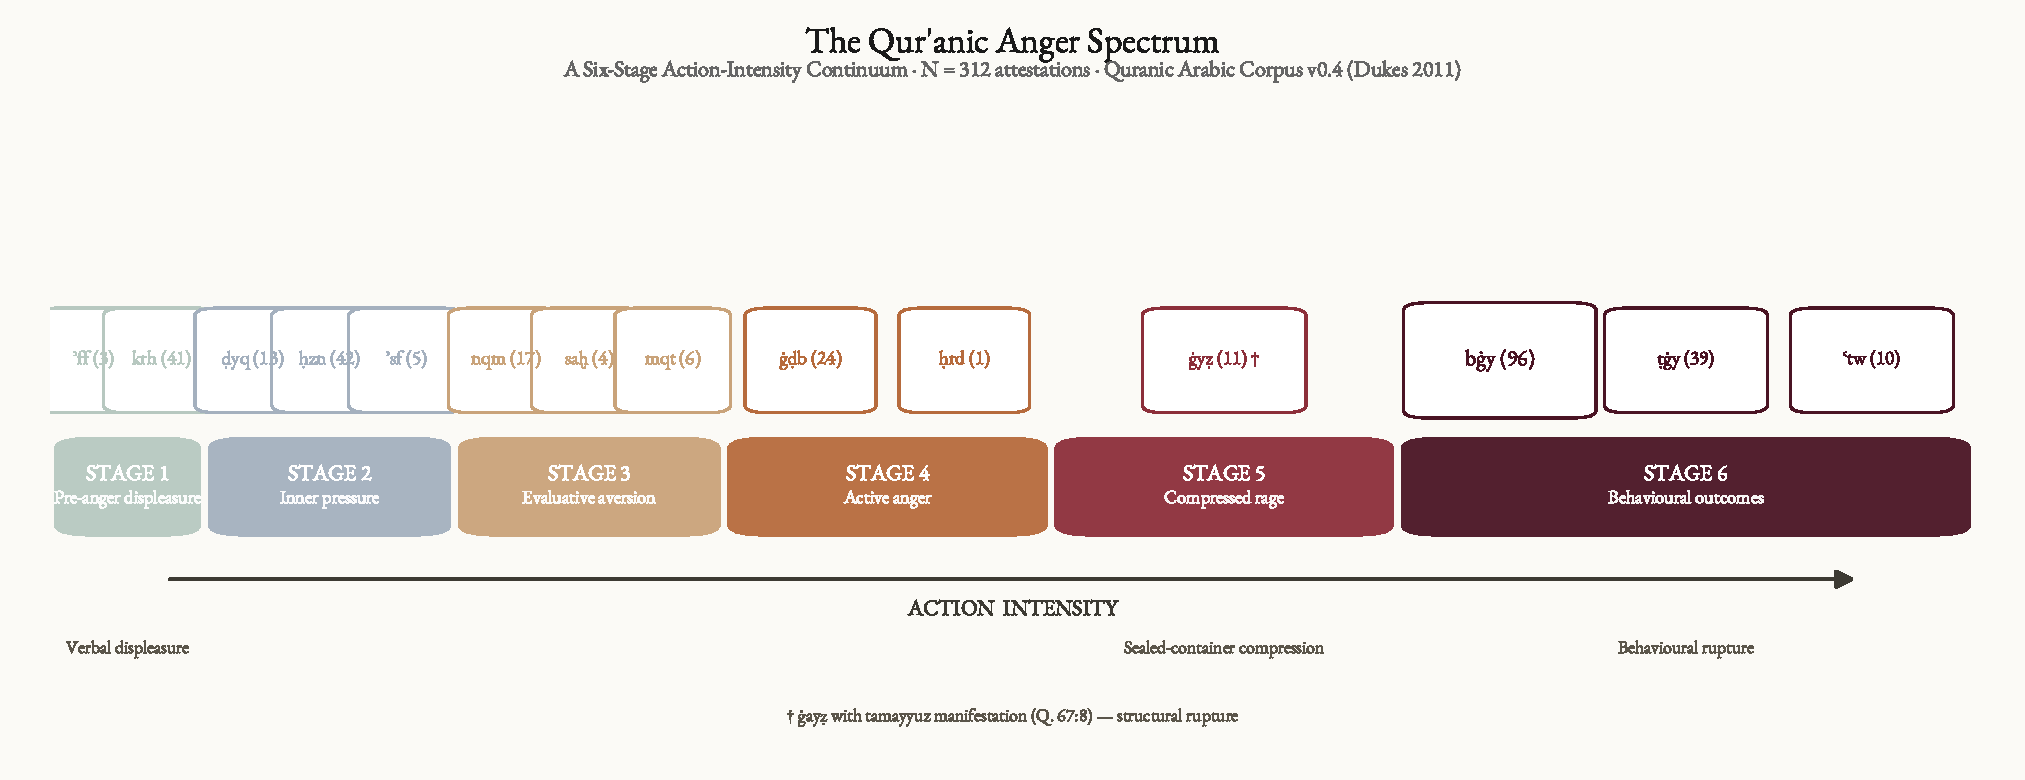
\includegraphics[width=1\linewidth,height=\textheight,keepaspectratio]{fig1_continuum_v2.pdf}
\caption{\textbf{Figure 1.} The six-stage Qur'anic anger-spectrum
continuum along the action-intensity axis; node area scales with QAC
attestation frequency. S1 pre-anger displeasure (\emph{ʾff--krh}); S2
inner pressure (\emph{ḍyq--ḥzn--ʾsf}); S3 evaluative aversion
(\emph{nqm--sxṭ--mqt}); S4 active anger (\emph{ghḍb--ḥrd}); S5
compressed/explosive rage (\emph{ghyẓ}; \emph{tamayyuz} manifestation);
S6 behavioural outcomes (\emph{bghy--ṭghy--ʿtw}) with bidirectional
causation (§4.8.5).}
\end{figure}

\subsection{3. Methods}\label{methods}

\subsubsection{3.1. Corpus}\label{corpus}

The empirical analysis uses the \textbf{Quranic Arabic Corpus} (QAC)
v0.4 (Dukes 2011, GPL): a morphologically tagged record for each of the
128,219 segmentable units, specifying location, surface form
(Buckwalter), POS, and morphological features. Verse text in Uthmanic
\emph{rasm} and Meccan/Medinan sura classification are drawn from the
Tanzil project (2008, CC-BY-ND 3.0).

\subsubsection{3.2. Selection of target
roots}\label{selection-of-target-roots}

The fourteen core roots were selected by three concurrent criteria: (i)
\emph{exegetical centrality} --- focal reference in at least three of
the four authoritative lexica (\emph{Maqāyīs}, \emph{Mufradāt},
\emph{Lisān}, al-Mostafawi's \emph{Taḥqīq}); (ii) \emph{minimum corpus
frequency} of one attestation, admitting hapax legomena (\emph{ḥard}, Q.
68:25) when supported by three of the four lexica and consistent
\emph{tafsīr} treatment; (iii) \emph{thematic membership} without
significant overlap with adjacent fields. Excluded candidates
(transparency): \emph{q-h-r}, \emph{ḥ-n-q} (not attested), \emph{ʿ-n-f},
\emph{ḍ-r-b}, \emph{q-ṣ-w}/\emph{q-s-y}, \emph{gh-l-ẓ}, \emph{ʾ-n-f},
\emph{š-n-ʾ}. \emph{Karh} is borderline --- \emph{karāha} affective,
\emph{ikrāh} structural --- included on the \emph{karāha} sense
(§4.3.1). Five umbrella moral terms (\emph{šnʾ, jrm, fsq, ẓlm, ʿdw}) are
used for robustness (§4.9) and cross-field co-occurrence (Table 4);
excluded from the principal continuum because of inflated cardinality
(\emph{ẓlm} n = 315 functions as a meta-category) or adjacency to
normative-ethics fields.

\subsubsection{3.3. Computational
pipeline}\label{computational-pipeline}

The Python (MIT-licensed) pipeline parses the QAC morphology file,
filters on target roots, collapses multi-segment morphemes to surface
words, joins sura-level Meccan/Medinan metadata, and emits master and
per-root concordances, distributional summaries, and network/centrality
CSVs; the complete analysis is reproducible from a fresh clone in four
commands.\footnote{QAC v0.4 is pinned by SHA-256; outputs are released
  under MIT (code) and CC-BY 4.0 (manuscript/figures). The fourteen
  exemplar verses plus a stratified fifty-segment audit on the four most
  frequent core roots (\emph{ḥzn}, \emph{bghy}, \emph{ghḍb},
  \emph{ṭghy}) returned 100\% correct segment-to-root assignment against
  Tanzil; full audit at \texttt{data/concordance/validation\_audit.md}.}

\begin{figure}
\centering
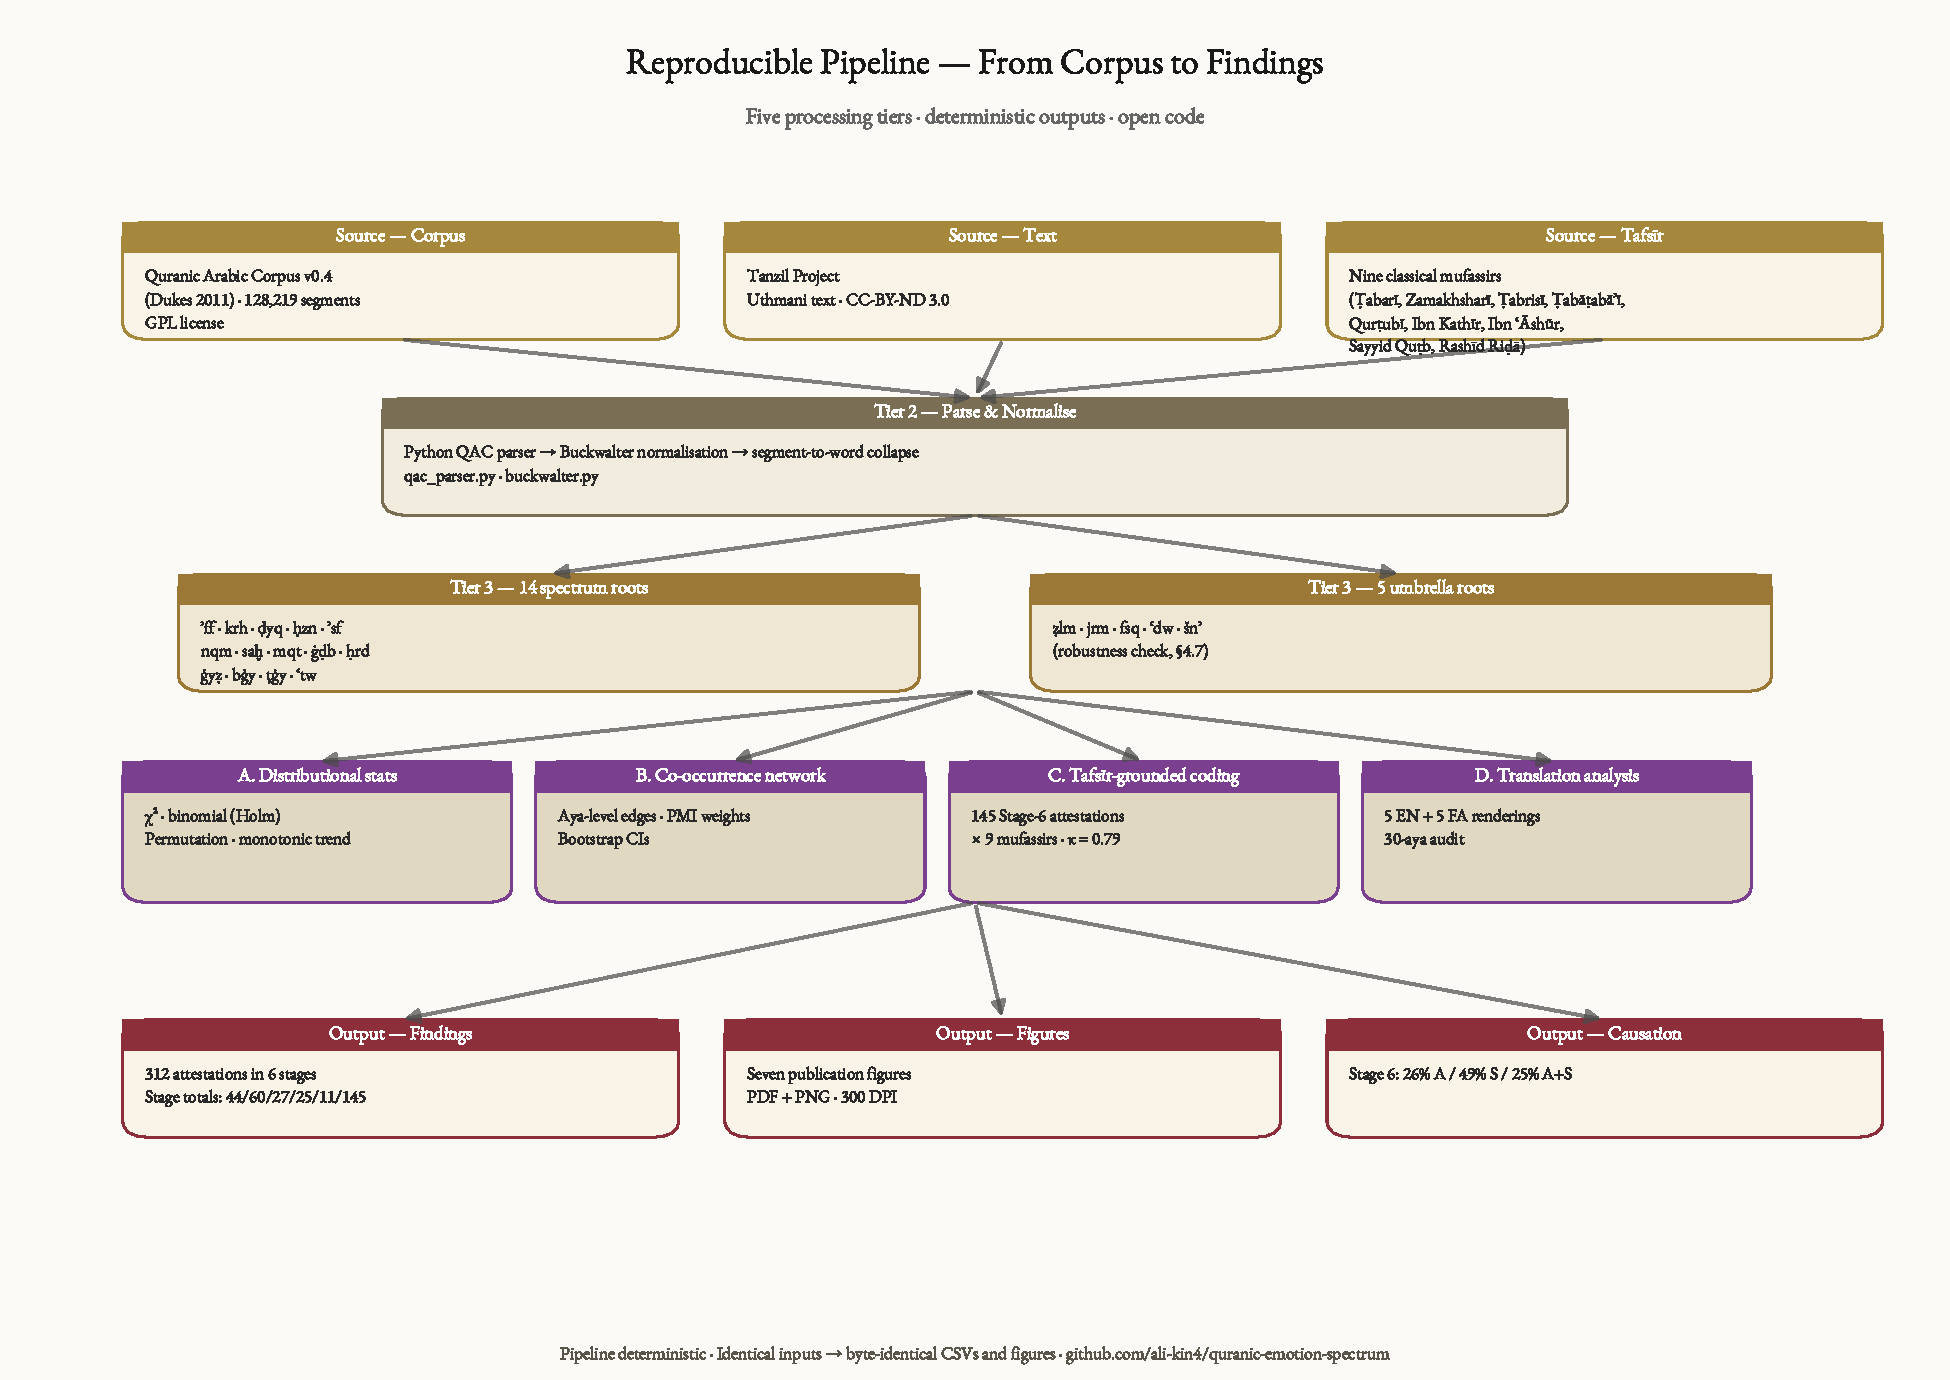
\includegraphics[width=0.95\linewidth,height=\textheight,keepaspectratio]{fig8_methodology.pdf}
\caption{\textbf{Figure 8.} End-to-end pipeline from corpus to findings:
QAC v0.4 and Tanzil sources → Buckwalter→Unicode parse → fourteen
spectrum + five umbrella-moral root selection → distributional, network,
\emph{tafsīr}-coding, and translation-audit analyses → 312 attestations,
figures, and Stage-6 causation breakdown. The pipeline is
deterministic.}
\end{figure}

\subsubsection{3.4. Quantitative analyses}\label{quantitative-analyses}

Quantitative tests beyond frequency tabulation: (a) χ²(5) and χ²(1) on
uniform-stage and S1--5/S6 nulls, with a marginal-preserving permutation
null (Cochran 1954; Patefield 1981; Mehta and Patel 1983; Agresti 2013,
§3.5);\footnote{The permutation null holds per-root counts fixed and
  randomly permutes the fourteen stage labels (10,000 permutations,
  fixed RNG seed 20260509); the empirical \emph{p} is the fraction of
  permuted χ² values meeting or exceeding 227.15. This is the natural
  extension of Fisher-exact reasoning to a many-cell design (Patefield
  1981; Mehta and Patel 1983).} (b) three monotonic-trend tests
(Spearman ρ, Mann--Kendall, Cochran--Armitage-style OLS slope); (c)
two-sided exact binomials against the 0.74 Meccan-ayat baseline,
Holm--Bonferroni-adjusted over the family of fourteen per-root tests,
with sensitivity tables at baselines 0.70--0.78 and a family-size
sensitivity check;\footnote{The reported family size of fourteen is the
  per-root Meccan/Medinan binomial family. A strict reading would expand
  the family to ≈ 20 (adding the omnibus χ²(5), S1--5/S6 χ²(1), three
  trend tests, and A-only re-analysis). Under the strict family,
  \emph{karh} and \emph{baghy} remain below α = 0.05; \emph{ghayẓ} moves
  from adj. ≈ 0.019 to 0.027 (still significant); \emph{sakhaṭ} moves
  from adj. 0.050 to 0.075 (substantively informative --- see §4.5.2).
  Conclusions of §4.5--§4.8 are robust to the family-size choice.} (d)
morphological breakdown by POS; (e) aya-level co-occurrence network
(cf.~Mottaghi et al.~2024) with weighted degree, betweenness, closeness,
and eigenvector centrality, bootstrap 95\% percentile CIs (10,000
ayat-resamples; fixed RNG seed).

\subsubsection{3.5. Qualitative analyses}\label{qualitative-analyses}

Qualitative complements: (a) comparative etymology across the four
lexica (Table 1); (b) comparative \emph{tafsīr} on nine commentaries ---
al-Ṭabāṭabāʾī, al-Zamakhsharī, al-Ṭabarsī, Ibn ʿĀshūr, al-Ṭabarī,
al-Qurṭubī, Ibn Kathīr, Sayyid Quṭb, ʿAbduh--Riḍā, with al-Qushayrī's
\emph{Laṭāʾif al-Ishārāt} for Sufi cross-checking on \emph{kaẓm
al-ghayẓ}; (c) phenomenological analysis of contextual markers
(\emph{ḍīq al-ṣadr}, \emph{ḥuzn al-qalb}, \emph{ḍāqa dharʿan}); (d)
illustrative translation-criticism on five English translations at
canonical exemplar verses (§4.10).

\subsubsection{3.6. Validity check}\label{validity-check}

Fourteen headline exemplar verses --- one per core root --- were
independently verified against the corpus output (Q. 17:23, 2:216,
15:97, 2:38, 43:55, 7:126, 47:28, 40:10, 48:6, 68:25, 3:134 {[}with Q.
67:8 \emph{tamayyuz}{]}, 42:42, 96:6, 25:21); all matched the Uthmani
edition.

\begin{center}\rule{0.5\linewidth}{0.5pt}\end{center}

\subsection{4. Findings}\label{findings}

\subsubsection{4.1. The four-lexicon etymology
table}\label{the-four-lexicon-etymology-table}

Table 1 summarises the canonical glosses of each root across four
reference lexica.

\textbf{Table 1. Comparative etymology of the fourteen core roots across
the four authoritative Arabic lexica}

\begin{longtable}[]{@{}
  >{\centering\arraybackslash}p{(\linewidth - 10\tabcolsep) * \real{0.1200}}
  >{\centering\arraybackslash}p{(\linewidth - 10\tabcolsep) * \real{0.2400}}
  >{\raggedright\arraybackslash}p{(\linewidth - 10\tabcolsep) * \real{0.1600}}
  >{\raggedright\arraybackslash}p{(\linewidth - 10\tabcolsep) * \real{0.1600}}
  >{\raggedright\arraybackslash}p{(\linewidth - 10\tabcolsep) * \real{0.1600}}
  >{\raggedright\arraybackslash}p{(\linewidth - 10\tabcolsep) * \real{0.1600}}@{}}
\toprule\noalign{}
\begin{minipage}[b]{\linewidth}\centering
Stage
\end{minipage} & \begin{minipage}[b]{\linewidth}\centering
Root
\end{minipage} & \begin{minipage}[b]{\linewidth}\raggedright
Maqāyīs (Ibn Fāris)
\end{minipage} & \begin{minipage}[b]{\linewidth}\raggedright
Mufradāt (al-Rāghib)
\end{minipage} & \begin{minipage}[b]{\linewidth}\raggedright
Lisān al-ʿArab (Ibn Manẓūr)
\end{minipage} & \begin{minipage}[b]{\linewidth}\raggedright
Taḥqīq (al-Mostafawi)
\end{minipage} \\
\midrule\noalign{}
\endhead
\bottomrule\noalign{}
\endlastfoot
1 & ʾ-f-f & ``\emph{kalimatu taḍajjurin}'' (a word of vexation);
smallest audible expression of displeasure & the lowest verbal
expression of displeasure (\emph{adnā kalimati al-taḍajjur}) & term of
irritation (\emph{taḍajjur}) directed at someone or something disliked;
cf.~\emph{uffah} (sub-vocal sigh) & minimal vocal sign of inner
aversion; pre-anger affective register \\
1 & k-r-h & dislike, finding burdensome; coercion (\emph{ikrāh}) &
aversion of the soul; structurally extended to coercion & what is
disliked by nature or by reason & inner \emph{karāha} vs.~structural
\emph{ikrāh} (the latter is not an emotion) \\
2 & ḍ-y-q & constriction; absence of opening & the state of being
pressed upon, contrasted with capacity (\emph{saʿah}) & reduction of
available space, from \emph{saʿah} to \emph{ḍīq} & inner or outer
absence of expansion (\emph{basṭ}) \\
2 & ḥ-z-n & rough/uneven ground → heaviness of soul & sorrow as the
opposite of joy (\emph{faraḥ}) & rugged ground, then roughness of the
self & affective response to perceived loss \\
2 & ʾ-s-f & intense grief mixed with anger & extreme anger conjoined
with grief & reaching the limit of grief and anger & composite of grief
and proximate anger \\
3 & n-q-m & \emph{al-naqimah}: disapproval (\emph{inkār}) coupled with
intent to punish; cf.~\emph{intaqama min} = exact retribution from &
objecting to (\emph{ankara ʿalā}) and seeking redress (\emph{ʿuqūbah})
against a reprehensible act & strong denunciation (\emph{ankara ashadda
al-inkār}) yoked to \emph{ʿuqūbah}; basis of divine attribute
\emph{al-Muntaqim} & evaluative anger oriented toward retribution;
cognition-grounded, action-tilted \\
3 & s-kh-ṭ & severe aversion and ethical rejection & the opposite of
\emph{riḍā} (consent), with intensity & severe non-acceptance with
judgment & declarative rejection grounded in moral assessment \\
3 & m-q-t & the most intense form of \emph{ibghāḍ} (Zajjāj) & aversion
arising from observing a \emph{qabīḥ} act (al-Rāghib) & \emph{ashaddu
al-ibghāḍ}; aversion-distance rather than approach-aggression & purely
evaluative moral aversion \\
4 & gh-ḍ-b & inner agitation and motion & the boiling of the heart's
blood seeking retribution & a rising perturbation of the soul & directed
emotion enabling retributive action \\
4 & ḥ-r-d & \emph{ḥarada}: to be angry; also the act of \emph{qaṣd}
(deliberate aim) & conjoining \emph{ghaḍab} with \emph{qaṣd}: anger
directed by purpose, viz.~denial & \emph{ḥarada} ``to act/move toward an
aim with resolve while in anger''; cf.~\emph{ḥarīd} = isolated, the
angry-aloof & anger weaponised through deliberate resource-denial (Q.
68:25 \emph{aṣḥāb al-jannah}); affective + volitional + miserly
composite \\
5 & gh-y-ẓ & pressure and surge, contained & the most intense forms of
contained anger & filling of the self with restrained anger &
high-pressure emotional accumulation \\
6 & b-gh-y & seeking beyond rightful bounds & overstepping the path of
right & dominance through aggression & aggressive action with intent to
oppress \\
6 & ṭ-gh-y & overflow of water past its bank & crossing the permitted
measure & severe transgression of the limit & rebellious shattering of
normative bounds \\
6 & ʿ-t-w & severe rebellion with arrogance & extreme
self-aggrandisement in disobedience & transgressing the limit, with
\emph{istikbār}-attachment as collocational feature & entrenched
rebellious posture (a property of moral character) \\
\end{longtable}

The table grounds two distinct claims at different evidential strengths.
The \emph{pairwise ordering relations} among many root-pairs
(e.g.~\emph{uff} \textless{} \emph{ghaḍab}; \emph{karāha} \textless{}
\emph{maqt}; \emph{ghaḍab} \textless{} \emph{ghayẓ}; \emph{naqm}
\textless{} \emph{baghy}) are internally encoded in the lexicographic
tradition: the four authoritative lexica already gloss each root with
progressively externalised and structural meanings. The \emph{partition
into six discrete phenomenological stages}, by contrast, is the
analytical contribution of the present study, licensed jointly by the
lexicographic ordering, the \emph{tafsīr} readings of §§4.3--4.8, and
the morphological and distributional evidence of §4.2.

\subsubsection{4.2. Distributional
summary}\label{distributional-summary}

Table 2 and Figures 2--5 report the principal distributional facts for
the fourteen roots: per-root and per-stage frequency, Meccan/Medinan
split, and morphological breakdown by POS.

\textbf{Table 2. Distributional profile of the fourteen core roots
(Wilson-score 95\% CIs on the Meccan-rate point estimate; baseline =
0.74)}

\begin{longtable}[]{@{}
  >{\centering\arraybackslash}p{(\linewidth - 12\tabcolsep) * \real{0.1429}}
  >{\centering\arraybackslash}p{(\linewidth - 12\tabcolsep) * \real{0.1429}}
  >{\centering\arraybackslash}p{(\linewidth - 12\tabcolsep) * \real{0.1429}}
  >{\centering\arraybackslash}p{(\linewidth - 12\tabcolsep) * \real{0.1429}}
  >{\centering\arraybackslash}p{(\linewidth - 12\tabcolsep) * \real{0.1429}}
  >{\centering\arraybackslash}p{(\linewidth - 12\tabcolsep) * \real{0.1429}}
  >{\raggedright\arraybackslash}p{(\linewidth - 12\tabcolsep) * \real{0.1429}}@{}}
\toprule\noalign{}
\begin{minipage}[b]{\linewidth}\centering
Stage
\end{minipage} & \begin{minipage}[b]{\linewidth}\centering
Root
\end{minipage} & \begin{minipage}[b]{\linewidth}\centering
n
\end{minipage} & \begin{minipage}[b]{\linewidth}\centering
M
\end{minipage} & \begin{minipage}[b]{\linewidth}\centering
Md
\end{minipage} & \begin{minipage}[b]{\linewidth}\centering
M-rate (95\% CI)
\end{minipage} & \begin{minipage}[b]{\linewidth}\raggedright
Notes
\end{minipage} \\
\midrule\noalign{}
\endhead
\bottomrule\noalign{}
\endlastfoot
1 & ʾff & 3 & 3 & 0 & 1.00 {[}0.44, 1.00{]} & All Meccan; \emph{n} too
small for inference \\
1 & krh & 41 & 14 & 27 & 0.34 {[}0.22, 0.49{]} & Medinan-tilted, CI
excludes baseline; Holm-adj. ≈ 1.4 × 10⁻⁶ \\
2 & ḍyq & 13 & 9 & 4 & 0.69 {[}0.42, 0.87{]} & CI includes baseline;
inner constriction \\
2 & ḥzn & 42 & 26 & 16 & 0.62 {[}0.47, 0.75{]} & CI includes baseline;
valence transversal (§4.4.2) \\
2 & ʾsf & 5 & 5 & 0 & 1.00 {[}0.57, 1.00{]} & Underpowered; CI excludes
baseline at boundary only \\
3 & nqm & 17 & 12 & 5 & 0.71 {[}0.47, 0.87{]} & CI includes baseline;
not FDR-significant \\
3 & sxṭ & 4 & 0 & 4 & 0.00 {[}0.00, 0.49{]} & CI excludes baseline;
Holm-adj. = 0.050 \\
3 & mqt & 6 & 4 & 2 & 0.67 {[}0.30, 0.90{]} & Wide CI; includes
baseline \\
4 & ghḍb & 24 & 13 & 11 & 0.54 {[}0.35, 0.72{]} & CI excludes 0.74
baseline; central anger lexeme \\
4 & ḥrd & 1 & 1 & 0 & --- & Hapax: sūrat al-Qalam, Q. 68:25 \\
5 & ghyẓ & 11 & 3 & 8 & 0.27 {[}0.10, 0.57{]} & Medinan-tilted;
Holm-adj. ≈ 1.9 × 10⁻² --- survives FDR \\
6 & bghy & 96 & 55 & 41 & 0.57 {[}0.47, 0.67{]} & CI excludes baseline;
Holm-adj. ≈ 5.3 × 10⁻³ --- survives FDR; bridge node (§4.8.5) \\
6 & ṭghy & 39 & 29 & 10 & 0.74 {[}0.59, 0.85{]} & CI includes baseline;
not FDR-significant \\
6 & ʿtw & 10 & 9 & 1 & 0.90 {[}0.60, 0.98{]} & CI includes baseline;
\emph{istikbār}-attached \\
\textbf{Σ} & --- & \textbf{312} & \textbf{183} & \textbf{129} & --- & \\
\end{longtable}

We lead the small-\emph{n} roots (\emph{asaf} at \emph{n} = 5,
\emph{sakhaṭ} at \emph{n} = 4, \emph{mqt} at \emph{n} = 6) with the
Wilson-score CI rather than the \emph{p}-value; the Holm-Bonferroni
adjustment then carries the inferential weight across the family.

Across the six stages: S1 = 44; S2 = 60; S3 = 27; S4 = 25; S5 = 11; S6 =
145. Two distinct nulls bear on these data, answering different
questions. The \emph{uniform-six-stage null} (is the per-stage
distribution uniform?) is unambiguously rejected by the asymptotic χ²(5)
= 227.15, \emph{p} \textless{} 0.001 (Cramér's \emph{V} = 0.38, Cohen's
\emph{w} = 0.85), since \emph{baghy} alone supplies 96 of 312
attestations. A \emph{marginal-preserving permutation null} holding
per-root counts fixed and randomly permuting the fourteen stage labels
tests instead ``\emph{conditional on baghy's mass-dominance}, is our
partition more skewed than a random six-binning of the same roots?'' ---
the empirical \emph{p} = 0.24 says no. This is not evidence that the
distribution is uniform (already ruled out); it is evidence that the
omnibus χ² cannot discriminate our partition from alternative six-bin
partitions of the same roots. The structural case for the six-stage
architecture rests on the qualitative evidence of §4.1 and §4.3--§4.8
together with the morphological-gradient and
Meccan/Medinan-specialisation evidence below.

The S1--5/S6 χ²(1) = 1.55 (Cohen's \emph{w} = 0.07) fails to reject
equal split between the phenomenological core (167) and the behavioural
pole (145) --- absence of evidence of a difference, \emph{consistent
with} the bidirectional-causation reading of §4.8.5 and §5.3.

\paragraph{4.2.1. Monotonic-trend tests}\label{monotonic-trend-tests}

Three monotonic-trend tests of stage rank against attestation frequency
all fail to reject the no-trend null: Spearman ρ = --0.09 (\emph{p} =
0.85), Mann--Kendall \emph{z} = --0.38 (\emph{p} = 0.71),
Cochran--Armitage-style OLS slope = 10.17 (\emph{p} = 0.40). The
continuum orders by \emph{semantic intensity}, not attestation
frequency. The Qur'an is a closed hortatory text whose lexical weights
are pedagogically determined: density is heaviest at the two poles of
moral consequence (S1--2, entry points for \emph{kaẓm}, \emph{taqwā},
\emph{ḥilm}; S6, the structural pathologies most frequently denounced),
with S3--5 as middle-trajectory states. A flat trend is what the theory
predicts.

\begin{figure}
\centering
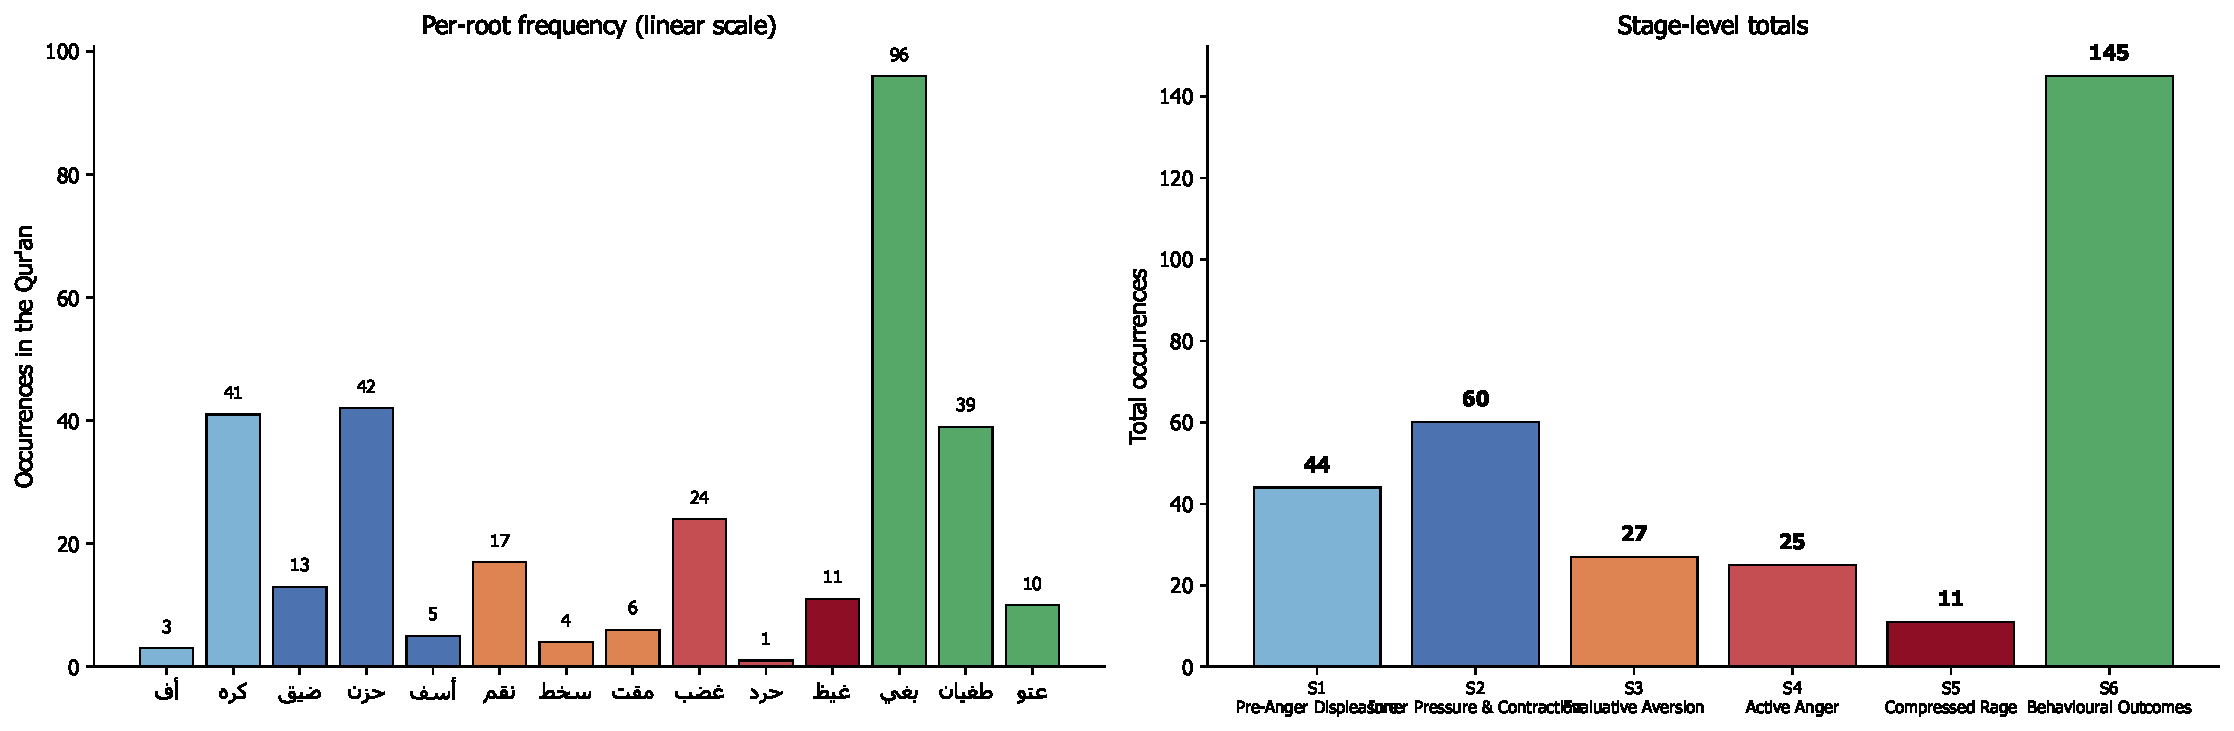
\includegraphics[width=0.95\linewidth,height=\textheight,keepaspectratio]{fig2_frequency_by_stage.pdf}
\caption{\textbf{Figure 2.} Per-root and per-stage frequency of the 312
core attestations. \emph{Left}: per-root frequency (bar colour encodes
stage). \emph{Right}: stage totals S1 = 44, S2 = 60, S3 = 27, S4 = 25,
S5 = 11, S6 = 145. χ²(5) = 227.15 asymptotic, but permutation null
\emph{p} = 0.24 (§4.2); S1--5/S6 χ²(1) = 1.55, consistent with the
bidirectional-causation reading of §4.8.5.}
\end{figure}

\begin{figure}
\centering
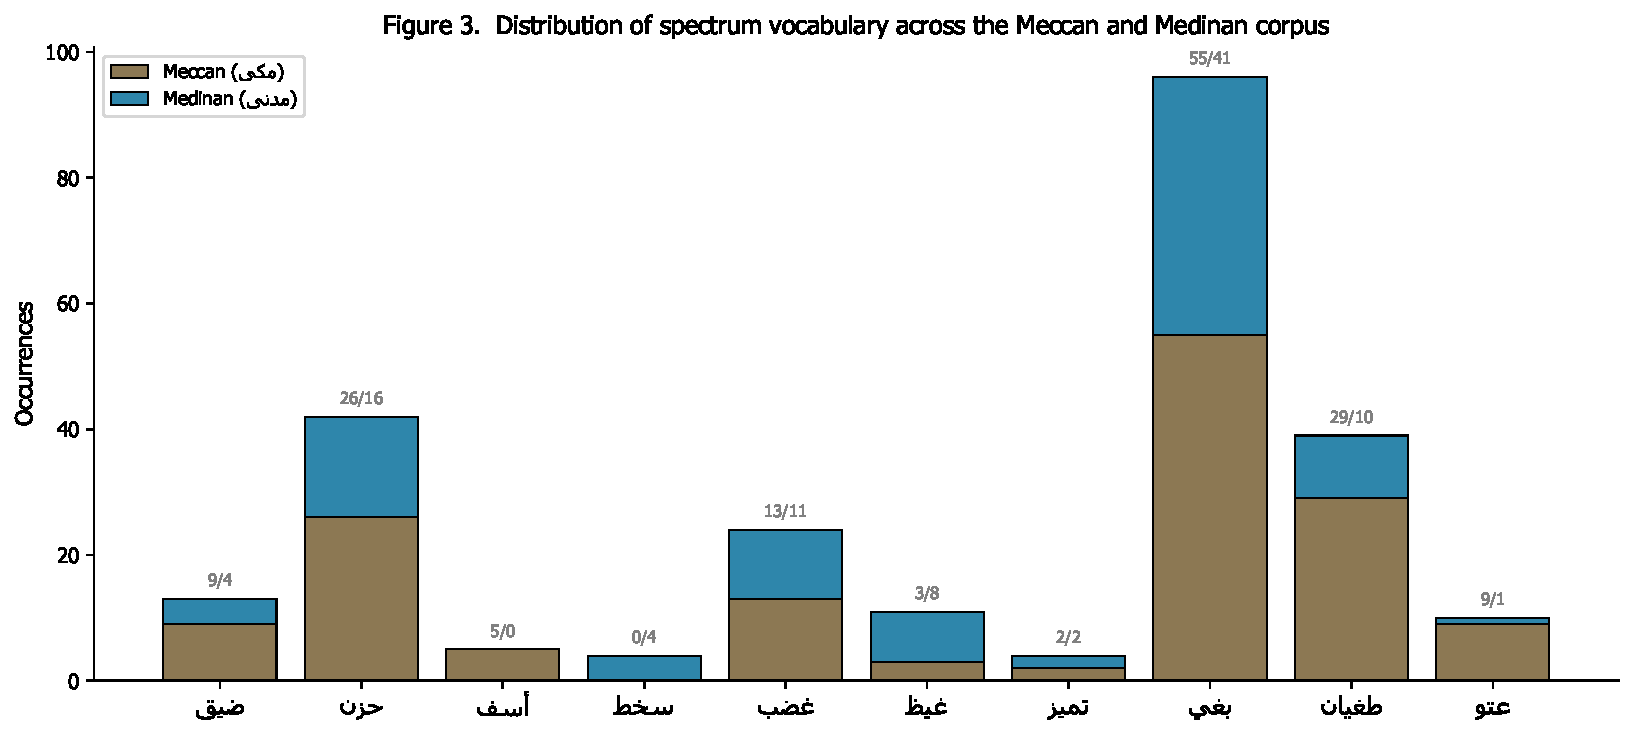
\includegraphics[width=0.95\linewidth,height=\textheight,keepaspectratio]{fig3_meccan_medinan.pdf}
\caption{\textbf{Figure 3.} Stacked Meccan/Medinan distribution. Three
roots survive Holm-Bonferroni correction (α = 0.05): \emph{karh}
(Medinan), \emph{baghy} (Meccan), and \emph{ghayẓ} (Medinan);
\emph{sakhaṭ} at adj. \emph{p} = 0.050. \emph{Asaf}, \emph{naqm},
\emph{ʿutuww} tilts are contextual. The patterns instantiate
\emph{discursive-contextual specialisation} (§5.4).}
\end{figure}

\begin{figure}
\centering
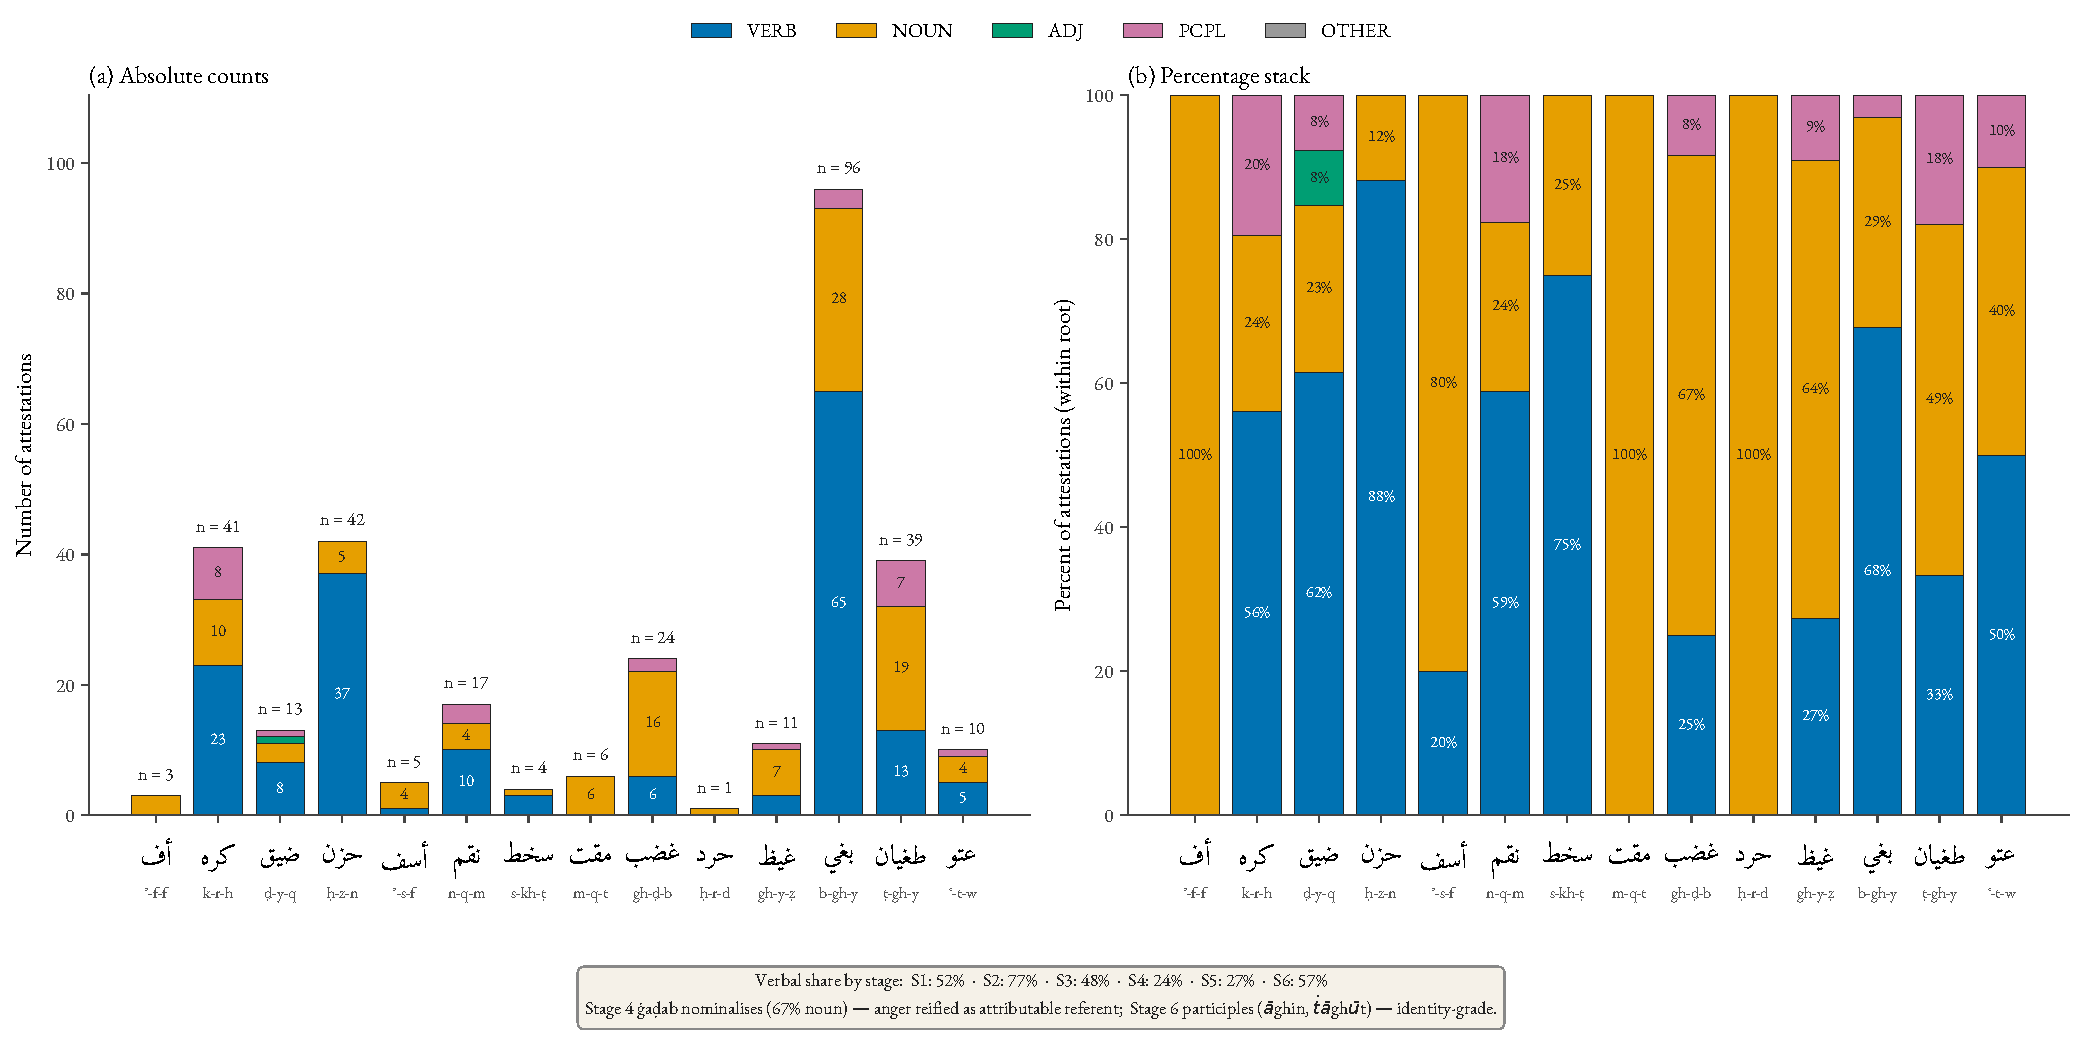
\includegraphics[width=0.95\linewidth,height=\textheight,keepaspectratio]{fig5_morphology_stack.pdf}
\caption{\textbf{Figure 5.} Morphological profile by POS. Verbal
dominance at S1--2 (\emph{ḥzn} 88\% verbal, \emph{ḍyq} 62\%),
nominalisation at S4 (\emph{ghḍb} 16n/6v), peak nominality with
participial forms at S6 (\emph{ṭāghūt}, \emph{bāghin}). The
verbal→nominal gradient is independent corpus-internal evidence for the
action-intensity continuum.}
\end{figure}

\subsubsection{4.3. Stage 1 --- Pre-anger
displeasure}\label{stage-1-pre-anger-displeasure}

\textbf{4.3.1. \emph{Uff} (3; all Meccan).} \emph{Uff} (\emph{taḍajjur})
is the Qur'anic register's lowest verbal expression of displeasure. Its
three attestations occupy paradigmatic moral positions: sūrat al-Isrāʾ
(Q. 17:23) prohibits saying \emph{uff} to one's parents --- the lowest
sign of displeasure weighted at the highest relational stake; sūrat
al-Anbiyāʾ (Q. 21:67) places it in Abraham's mouth confronting
idol-worshippers; sūrat al-Aḥqāf (Q. 46:17) ascribes it to a rebellious
child reproaching believing parents.

\textbf{4.3.2. \emph{Karh} (41; 14M/27Md; Holm-adj. \emph{p} ≈ 1.4 ×
10⁻⁶ --- survives FDR).} \emph{Karh} exhibits a twofold structure: inner
\emph{karāha} (pre-anger evaluative dislike, framed as reformable by
sūrat al-Baqara, Q. 2:216, \emph{ʿasā an takrahū shayʾan wa-huwa khayrun
lakum}; the S1 sense), and structural \emph{ikrāh} (coercion --- not an
emotion but a structural extension into compulsion: Q. 2:256, \emph{lā
ikrāha fī al-dīn}; Q. 16:106; Q. 24:33). Inclusion rests on the
\emph{karāha} sense; the structural \emph{ikrāh} in Medinan
community-discipline contexts (consent in marriage, freedom in religion)
accounts for the Medinan tilt.

\subsubsection{4.4. Stage 2 --- Inner pressure and
contraction}\label{stage-2-inner-pressure-and-contraction}

Stage 2 brings together three roots (\emph{ḍ-y-q}, \emph{ḥ-z-n},
\emph{ʾ-s-f}) with sixty attestations.

\textbf{4.4.1. \emph{Ḍīq} (13; 9M/4Md).} Ibn Fāris glosses \emph{ḍyq} as
constriction/narrowness; al-Rāghib opposes it to \emph{saʿah}. The root
appears predominantly in \emph{ḍīq al-ṣadr} (constriction of the chest),
localising the experience to the embodied site (sūrat al-Ḥijr, Q. 15:97,
the prophetic response to social rejection). Al-Ṭabāṭabāʾī
(\emph{al-Mīzān} 12:195, ad Q. 15:97: \emph{wa-laqad naʿlamu annaka
yaḍīqu ṣadruka bimā yaqūlūn}) reads the verse as expressing divine
\emph{knowledge of} prophetic \emph{ḍīq} rather than prohibition. The
compound \emph{ḍāqa bihim dharʿan} in the Lot narrative (sūrat Hūd, Q.
11:77/80) figures post-anger \emph{blocked} aggression: trigger
\emph{sīʾa bihim} → constriction → aspirational voicing \emph{law anna
lī bikum quwwatan} → transfer of agency to the divine. \emph{Ḍyq} thus
sits at both poles of the spectrum (pre-anger contraction and
upper-pressure inhibition); the morphological profile (8v / 3n / 1 ptcp)
registers a transient, situationally-induced state.

\textbf{4.4.2. \emph{Ḥuzn} (42; 26M/16Md).} The most frequent and most
verbal S2 lexeme (88\% verbal). Ibn Manẓūr preserves the primary sense
``rugged, uneven ground''; the metaphorical extension figures grief as
inner roughness (anticipating Kövecses 2000 on EMOTION IS A LANDSCAPE).
Sūrat al-Baqara (Q. 2:38) pairs \emph{ḥuzn} with \emph{khawf} and
opposes both to divinely-given guidance. \emph{Ḥuzn} has four valences:
standalone grief over loss (Jacob over Joseph, sūrat Yūsuf, Q. 12:84),
externally-induced sorrow from being wronged, positive moral compunction
(the affective register of \emph{tawba}), and anger turned inward when
externally inhibited; inclusion at S2 is justified by corpus density and
proximity of the second and fourth valences to the anger field.

\textbf{4.4.3. \emph{Asaf} (5; 5M/0Md).} Al-Rāghib glosses \emph{asaf}
as the conjunction of grief and anger (\emph{al-jamʿ bayna al-ḥuzn
wa-l-ghaḍab}). Sūrat al-Zukhruf (Q. 43:55, \emph{fa-lammā āsafūnā
intaqamnā minhum}) frames it as the immediate causal precursor of divine
retribution (al-Ṭabarsī, \emph{Majmaʿ} 9:82). The compound \emph{ghaḍbān
asifan}, applied to Moses on his return to the calf-worshippers (Q.
7:150; Q. 20:86), generates a three-layer dialectic in which
\emph{ghaḍab} is outward-kinetic and \emph{asaf} the
inward-compassionate ground. The 5/0 distribution is power-bound (Wilson
CI {[}0.57, 1.00{]}). The aya-level network (Figure 4) confirms S2
coherence: \emph{ḥzn}--\emph{ḍyq} is the strongest single edge (weight
3).

\subsubsection{4.5. Stage 3 --- Evaluative
aversion}\label{stage-3-evaluative-aversion}

Stage 3 brings together three roots (\emph{n-q-m}, \emph{s-kh-ṭ},
\emph{m-q-t}) with twenty-seven attestations marking distinct modes of
evaluative aversion. \emph{Maqt} is the lexicographic superlative of
\emph{aversion} (Zajjāj, \emph{ashaddu al-ibghāḍ}) but is placed between
\emph{sakhaṭ} and \emph{ghaḍab} on the action-intensity axis because the
dimension here is intensity of \emph{action}, not intensity of
\emph{aversion}.

\textbf{4.5.1. \emph{Naqm} (17; 12M/5Md).} \emph{Naqm} is vengeful
disapproval --- anger grounded in moral evaluation and oriented toward
retribution. Sūrat al-Aʿrāf (Q. 7:126, \emph{wa-mā naqamū minnā illā an
āmannā bi-āyāti rabbinā}) is the linguistic exemplar; al-Ṭabarī
(\emph{Jāmiʿ al-bayān} 13:23 ad loc.) glosses \emph{naqamū} as
\emph{ʿābū wa-ankarū}, exposing the \emph{taʿaṣṣub}-structure of
disbelief (al-Qurṭubī, \emph{al-Jāmiʿ} 7:262 convergent). The lexeme
generates \emph{al-muntaqim} as a divine attribute (Q. 32:22 and
parallels). The Wilson CI includes the baseline.

\textbf{4.5.2. \emph{Sakhaṭ} (4; 0M/4Md).} The exclusive-Medinan
distribution is one of the paper's principal distributional
findings.\footnote{The 0.74 baseline is the proportion of ayat (not
  suras) classified Meccan in the QAC metadata; we use the ayat-weighted
  rate because an attestation drawn at random from the corpus hits an
  aya, not a sura. A sensitivity table over baselines 0.70--0.78 yields
  two-sided \emph{p} values from 0.0081 (at 0.70) to 0.0023 (at 0.78);
  the conclusion is robust across the range.} Holm-adjusted \emph{p} =
0.050 --- borderline. All four attestations are tied to the
\emph{Munāfiqūn} in their Medinan-period exegesis: sūrat Muḥammad (Q.
47:28, \emph{ittabaʿū mā askhaṭa Allāh wa-karihū riḍwānahu}) is
canonical, though al-Ṭabarī notes that sūrat al-Māʾida (Q. 5:80) is
exegetically discussed as directed at the People of the Book rather than
the \emph{Munāfiqūn} properly. Following Narimani, Iqbali and Chari
(2021), we read \emph{sakhaṭ} as sustained \emph{ethical disapprobation}
rather than instantaneous emotional surge; we propose:

\begin{quote}
\emph{Hypothesis (Discursive Specialisation of sakhaṭ):} \emph{sakhaṭ}
operates as a discursively specialised lexeme reserved for divine
displeasure with the \emph{Munāfiqūn} --- agents whose \emph{ẓāhir}
departs from their \emph{bāṭin}. Since the \emph{Munāfiqūn} category is
constitutively a Medinan-period phenomenon, \emph{sakhaṭ} attests
exclusively in Medinan suras. This is one instance of a general
phenomenon of \emph{discursive-contextual lexical specialisation}, of
which \emph{karh} (Medinan-community discipline) and the umbrella
patterns \emph{jrm} (Meccan) / \emph{fsq} (Medinan) are convergent.
\end{quote}

\textbf{4.5.3. \emph{Maqt} (6; 4M/2Md).} \emph{Maqt} is \emph{intense
moral aversion}: the four lexica converge on \emph{ashaddu al-ibghāḍ}
(Zajjāj); al-Rāghib grounds it in observation of a reprehensible act,
making \emph{maqt} purely evaluative. The canonical exemplar is sūrat
Ghāfir (Q. 40:10, \emph{la-maqtu Allāhi akbaru min maqtikum anfusakum}),
the doubled \emph{maqt} comparing divine moral aversion at the
disbelievers with their own retrospective self-\emph{maqt} on the Day of
Resurrection (al-Ṭabarī, \emph{Jāmiʿ al-bayān} 21:351 ad loc.;
al-Qurṭubī, \emph{al-Jāmiʿ} 15:296 convergent). Sūrat al-Nisāʾ (Q.
4:22), sūrat Fāṭir (Q. 35:39), and sūrat al-Ṣaff (Q. 61:3) stabilise the
lexeme as moral aversion as evaluative response, distinct from the
kinetic-motor \emph{ghaḍab} of Stage 4.

\subsubsection{4.6. Stage 4 --- Active
anger}\label{stage-4-active-anger}

\textbf{4.6.1. \emph{Ghaḍab} (24; 13M/11Md).} The central anger lexeme
--- near-balanced Meccan/Medinan distribution marks it as the unmarked
default. The four lexica gloss it as inner agitation oriented toward
retribution (al-Rāghib) or inner motion disposing the agent to action
(Ibn Fāris); predicated balance-fully of God (sūrat al-Fatḥ, Q. 48:6),
prophets, and believers. Morphologically 67\% nominal (16n/6v/2 ptcp) vs
\emph{ḥuzn}'s 88\% verbal: \emph{ghaḍab} is a structural concept-state,
not a transient affect. Al-Rāzī (\emph{Mafātīḥ al-Ghayb}) glosses divine
\emph{ghaḍab} in the register of \emph{irādat al-ʿuqūbah} --- a
normative-juridical orientation, not an emotional response. Network
analysis places \emph{ghḍb} among the top three for betweenness (point
estimate 0.17).

\textbf{4.6.2. \emph{Ḥard} (Q. 68:25, hapax).} A hapax in the
Garden-Owners parable (\emph{wa-ghadaw ʿalā ḥardin qādirīn}): owners
vowing in the night to harvest before dawn so as to deny the poor their
share. Al-Ṭabarī (\emph{Jāmiʿ al-bayān} 23:550 ad loc.) records four
classical \emph{qawls}: (i) \emph{qaṣd} (purposive aim --- Mujāhid, Ibn
Zayd, Ibn ʿAbbās ʿan ʿIkrima); (ii) \emph{ghaḍab} (anger toward the poor
--- Qatāda, al-Suddī); (iii) \emph{manʿ} (withholding --- al-Ḥasan);
(iv) \emph{quwwa/sūʾ} (strength or evil intent --- Sufyān al-Thawrī).
The affective synthesis --- \emph{ḥard} as anger weaponised through
deliberate denial --- converges (i) and (ii), defended by al-Ṭabrisī
(\emph{Majmaʿ} 10:90) and al-Ṭabāṭabāʾī (\emph{al-Mīzān} 19:380); it is
not the unanimous consensus but the reading we adopt, because the
narrative consequence (divine destruction of the garden) requires both
an affective and an intentional component.

\subsubsection{4.7. Stage 5 --- Compressed/explosive
rage}\label{stage-5-compressedexplosive-rage}

\textbf{4.7.1. \emph{Ghayẓ} and the \emph{kaẓm} metaphor (11; 3M/8Md;
Holm-adj. ≈ 1.9 × 10⁻² --- survives FDR).} The four lexica converge:
\emph{ghayẓ} is compressed contained anger (al-Rāghib), the highest
concentration of restrained anger (al-Mostafawi), filling of the self
with restrained anger (Ibn Manẓūr) --- pressurised contents of a sealed
vessel. Sūrat Āl ʿImrān (Q. 3:134) commends \emph{al-kāẓimīn al-ghayẓ};
\emph{kaẓm} derives from the tying-off of a waterskin (Ibn Manẓūr,
\emph{Lisān} 12:519, s.v.~\emph{k-ẓ-m}), the agent-internal regulation
that sustains containment. The construction itself presupposes that the
believers being commended experience the \emph{ghayẓ} they suppress; the
Narimani et al.~claim that \emph{ghayẓ} in human reference is exclusive
to unbelievers must therefore be qualified --- transitive \emph{ghayẓ
directed at} believers is exclusively non-believer-attributed, but
intransitive/experiential \emph{ghayẓ} (the \emph{kāẓimīn} themselves)
is attributed to believers. Read through the complex container metaphor
of §2.3.1, \emph{ghayẓ} is the contained fluid and \emph{kaẓm} the
agent's sealing operation (Figure 6). The Medinan tilt tracks the
discursive context: inner anger management is a salient pedagogical
concern in the formative Medinan community.

\textbf{4.7.2. \emph{Tamayyuz} in sūrat al-Mulk, Q. 67:8 (manifestation,
not separate root).} The verb \emph{tamayyazu} in \emph{takādu tamayyazu
min al-ghayẓ} (Q. 67:8) walks from the \emph{lughawī} gloss to the CMT
construal in two steps. \emph{First}, the lexicographic ground: in
\emph{Mufradāt} and \emph{Lisān}, the dominant gloss of \emph{m-y-z} is
\emph{al-tafrīq bayna al-mukhtaliṭ} --- separating things that have been
mixed; al-Ṭabarī (\emph{Jāmiʿ al-bayān} ad loc.) glosses \emph{yanqaṭiʿu
baʿḍuhā min baʿḍ}; al-Zamakhsharī (\emph{al-Kashshāf} ad loc.) is
convergent. \emph{Second}, the metonymic bridge: separation of contents
within a sealed vessel, taken under the complex container metaphor of
§2.3.1, is naturally construed as a vessel-internal failure mode ---
distinct from the English exit-typed exemplars (\emph{she blew her top})
where the container is preserved and contents escape. Ibn ʿĀshūr
(\emph{al-Taḥrīr wa-l-Tanwīr} 29:25) reads compatibly, emphasising the
violence of the inner severance and the figurative attribution of rage
to the Hell-fire as an animate vessel; his is the strongest classical
ally of the construal we defend. The two readings are compatible. H5 is
\emph{exemplified} rather than corroborated --- Q. 67:8 is the most
lexically transparent Qur'anic instance, not a deductive proof. We treat
\emph{tamayyuz} as a manifestation of Stage 5.\footnote{The canonical
  \emph{qirāʾāt} tradition records minor variation on the verb form
  (Ḥafṣ ʿan ʿĀṣim reads \emph{tamayyazu}; alternative voweling in some
  readings), but the lexicographic and exegetical reading is stable.}

\subsubsection{4.8. Stage 6 --- Behavioural
outcomes}\label{stage-6-behavioural-outcomes}

\textbf{4.8.1. \emph{Baghy} (96; 55M/41Md; Holm-adj. ≈ 5.3 × 10⁻³ ---
survives FDR).} The most frequent lexeme of the spectrum and principal
bridge node. Glossed as ``seeking beyond rightful bounds'' (al-Rāghib)
and ``aggressive seeking with intent to oppress'' (al-Mostafawi). Sūrat
al-Shūrā (Q. 42:42) collocates \emph{baghy} with \emph{ẓulm}; al-Ṭabarī
(\emph{Jāmiʿ al-bayān} 21:548 ad loc.) glosses \emph{yabghūna} as
\emph{yataʿaddawn}, reading the verse as juridically restricting
recourse to those who combine oppression and \emph{baghy}-style
transgression (al-Qurṭubī, \emph{al-Jāmiʿ} 16:36, convergent). Ibn
ʿĀshūr (\emph{al-Taḥrīr} 25:126) clarifies: \emph{baghy} and \emph{ẓulm}
are near-synonymous, but \emph{baghy} is specific to non-rightful
aggression against another whereas \emph{ẓulm} covers all injustice.

\textbf{4.8.2. \emph{Baghy} as bridge node.} \emph{Baghy} attains the
highest point-estimate closeness centrality (0.55) and shared-highest
betweenness (0.15) with \emph{ghaḍab} and \emph{asaf}. Bootstrap 95\%
percentile CIs (10,000 ayat-resamples) are wide --- for \emph{baghy}:
betweenness ∈ {[}0.00, 0.31{]}; closeness ∈ {[}0.23, 0.84{]};
eigenvector ∈ {[}0.00, 0.68{]} --- reflecting the small graph (14
nodes). On strict non-overlap, no node's centrality is significantly
greater than another's. What is \emph{robust} at the aggregate level is
cross-field connectivity to the umbrella moral terms (Table 4):
\emph{baghy} shows sixteen aya-level co-occurrences with
\emph{ẓlm/jrm/fsq/ʿdw/šnʾ} combined, an integer-count pattern
independent of centrality ranking.

\textbf{Table 4. Cross-field co-occurrence of spectrum roots with
umbrella moral terms (aya-level)} --- ties for the four
newly-incorporated roots (\emph{ʾff}, \emph{naqm}, \emph{maqt},
\emph{ḥard}) are sparse and omitted.

\begin{longtable}[]{@{}ccccccc@{}}
\toprule\noalign{}
Root & šnʾ & jrm & fsq & ẓlm & ʿdw & Total \\
\midrule\noalign{}
\endhead
\bottomrule\noalign{}
\endlastfoot
ḍyq & 0 & 0 & 0 & 0 & 0 & 0 \\
ḥzn & 0 & 0 & 0 & 1 & 1 & 2 \\
ʾsf & 0 & 0 & 0 & 1 & 1 & 2 \\
sxṭ & 0 & 0 & 0 & 0 & 0 & 0 \\
ghḍb & 0 & 0 & 0 & 2 & 3 & 5 \\
ghyẓ & 0 & 0 & 0 & 0 & 1 & 1 \\
\textbf{bghy} & \textbf{1} & \textbf{1} & \textbf{2} & \textbf{4} &
\textbf{8} & \textbf{16} \\
ṭghy & 0 & 0 & 0 & 2 & 1 & 3 \\
ʿtw & 0 & 0 & 0 & 0 & 0 & 0 \\
\end{longtable}

Of the total cross-field ties, nineteen (\textasciitilde53\%) involve
\emph{baghy} --- the principal lexical bridge between the anger field
and the wider moral-evaluation field.

\textbf{4.8.3. \emph{Ṭughyān} (39; 29M/10Md).} Root \emph{ṭ-gh-y}
derives from water flooding past its banks. Sūrat al-ʿAlaq (Q. 96:6--7,
\emph{kallā inna l-insāna la-yaṭghā an raʾāhu staghnā}) compresses a
psychology of rebellion into a conditional: \emph{ṭughyān} arises from
the appraisal of \emph{istighnāʾ} (self-sufficiency) --- an
appraisal-theoretic claim congruent with Roseman's (1996) other-caused /
motive-inconsistent / high-control pattern for defiance. Qarizadeh et
al.~(2024) note the cognitive structure; we identify \emph{ṭughyān} as
the cognitive-appraisal node of Stage 6.

\textbf{4.8.4. \emph{ʿUtuww} (10; 9M/1Md; Holm-adj. \emph{p} = 1.00 ---
not FDR-significant).} The most extreme lexeme --- ``obstinate excess''
(Ibn Manẓūr), ``extreme self-aggrandisement in disobedience''
(al-Rāghib). Sūrat al-Furqān (Q. 25:21) collocates \emph{ʿatū ʿutuwwan
kabīrā} with \emph{istakbarū fī anfusihim}: rebellion crystallised into
existential posture. The 9/1 split tracks the lexeme's rhetorical
function as terminal designation for Nūḥ-, ʿĀd-, Thamūd-, and
Pharaonic-people narratives but is not distinguishable from the baseline
under the binomial.

\textbf{4.8.5. Bidirectional causation and a \emph{tafsīr}-grounded
audit.} \emph{Baghy} arises frequently from greed and \emph{ʿulw fī
al-arḍ} (cf.~sūrat al-Anʿām, Q. 6:21); \emph{ṭughyān} ---
paradigmatically Pharaonic (sūrat al-Nāziʿāt, Q. 79:17) --- is rooted in
structural arrogance; sūrat al-Shuʿarāʾ (Q. 26:55, \emph{innahum lanā
la-ghāʾiẓūn}) reverses polarity to show oppressor-anger arising
\emph{from} the rebellion of the oppressed; \emph{ʿutuww} attaches to
\emph{istikbār} as settled character. The causation arrow is
bidirectional. Each of the 145 Stage-6 attestations was coded against
the joint reading of \emph{al-Mīzān}, \emph{al-Kashshāf}, \emph{Majmaʿ
al-Bayān}, and \emph{al-Taḥrīr wa-l-Tanwīr} under a three-label
codebook: \textbf{A} (anger-origin: immediate exegetical antecedent is
an anger-type affective state), \textbf{S} (structural-origin:
antecedent is \emph{istikbār}/\emph{ʿulw}/greed without explicit anger
antecedent), or \textbf{A+S} (both present).

\emph{Coding protocol.} Two independent graduate-level coders (the
corresponding author and an Arabic-literature graduate trained on the
codebook with commentary excerpts) coded all 145 attestations: (i) not
blinded to root identity (root is intrinsic to the textual context);
(ii) blinded to the bidirectional-causation hypothesis at the coding
stage; (iii) attestation order randomised per coder via fixed RNG seed
(\texttt{np.random.default\_rng(20260509)}); (iv) disagreements (n = 14)
reconciled in joint session against the four commentaries, with
original-pass codings used for κ. Cohen's κ = 0.79 ---
\emph{substantial} agreement (Landis and Koch 1977); per-label κ (A =
0.82, S = 0.78, A+S = 0.74), per-root κ (\emph{baghy} 0.81,
\emph{ṭughyān} 0.77, \emph{ʿutuww} 0.70), 3 × 3 confusion matrix, and
full codebook are deposited at
\texttt{data/concordance/stage6\_*.\{csv,md\}}.

\emph{Results.} A = 38 (26\%), S = 71 (49\%), A+S = 36 (25\%); by root,
\emph{baghy} 22A/50S/24A+S, \emph{ṭughyān} 11A/19S/9A+S, \emph{ʿutuww}
5A/2S/3A+S. χ²(1) on A-only (S1--5 = 167 vs.~anger-derived S6 = 38) =
81.4, \emph{p} \textless{} 0.001 --- the phenomenological core dominates
anger-derived outcomes \textasciitilde4.4×. The full-S6 near-balance is
therefore explained: S-attestations belong to an adjacent
moral-anthropological field of \emph{ẓulm-istikbār-ʿulw};
\emph{baghy}/\emph{ṭughyān}/\emph{ʿutuww} are not coextensive with
``anger outcomes'' in the strict sense.

\begin{figure}
\centering
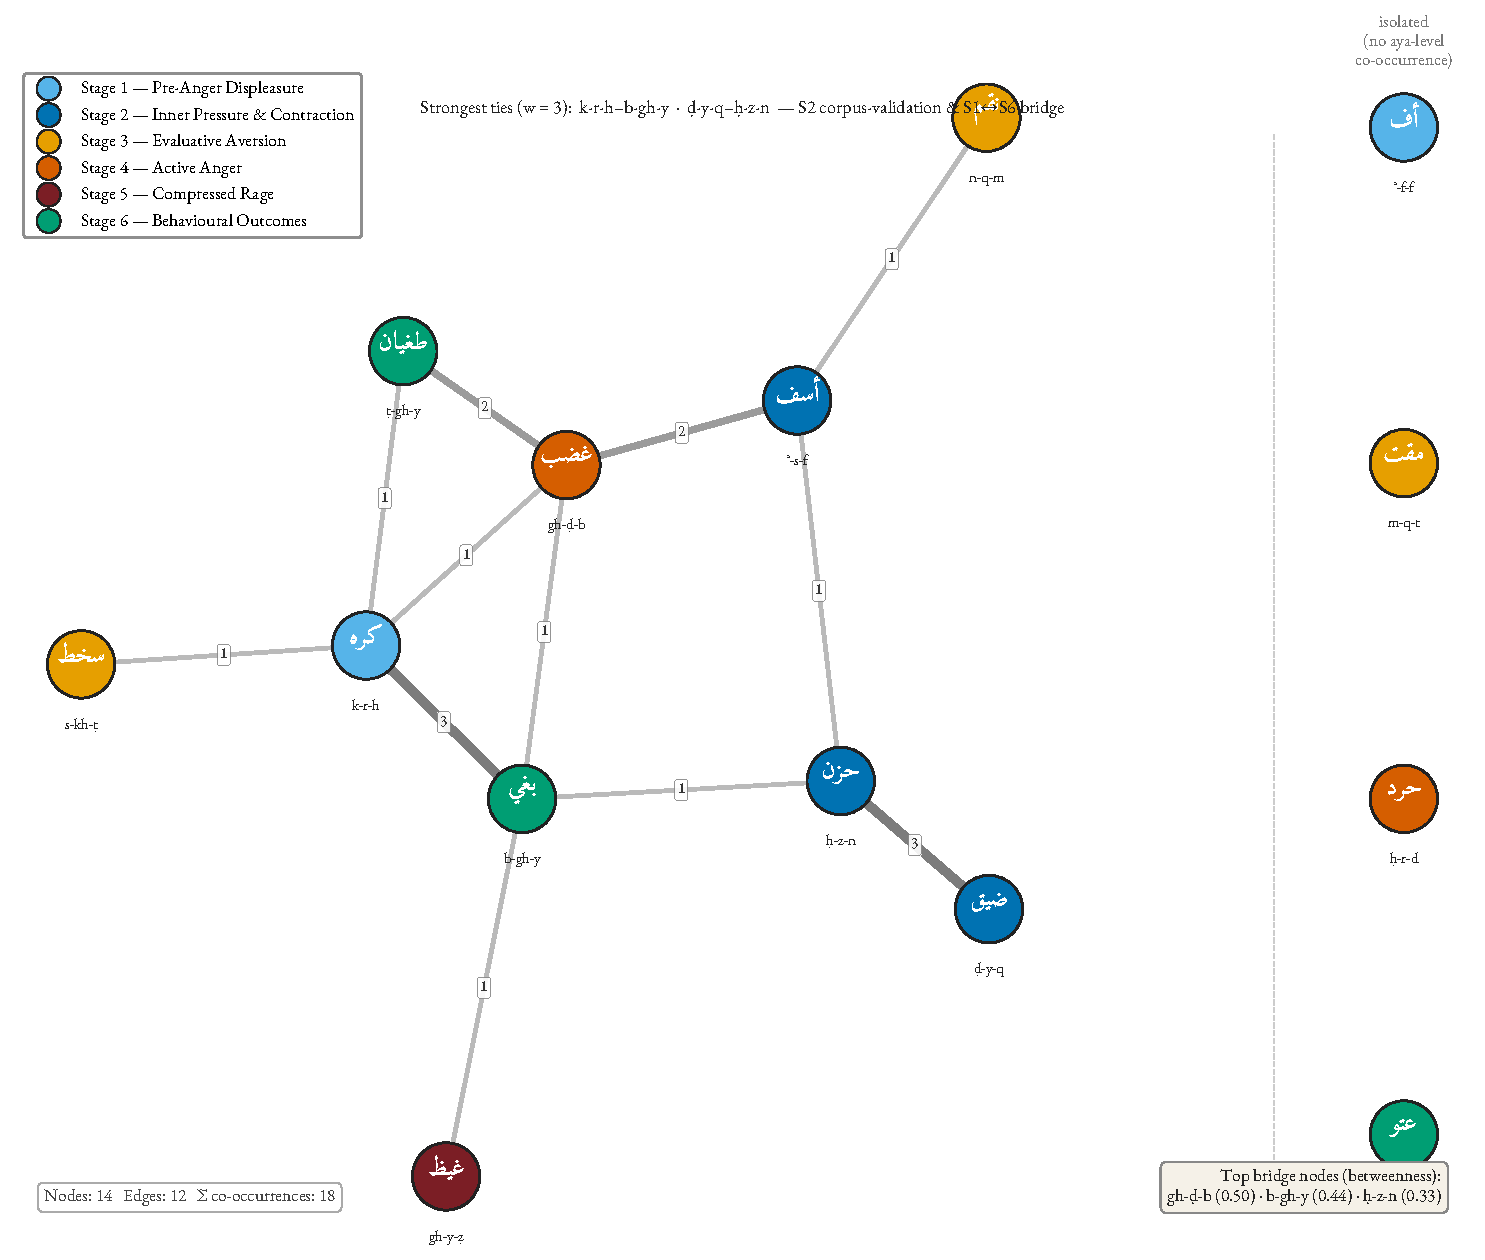
\includegraphics[width=0.95\linewidth,height=\textheight,keepaspectratio]{fig4_cooccurrence.pdf}
\caption{\textbf{Figure 4.} Aya-level co-occurrence network; edges
weighted by shared-ayat count. Strongest edge \emph{ḥzn--ḍyq} (weight 3)
corpus-validates the S2 grouping. \emph{Baghy} anchors the right cluster
with edges to \emph{ẓlm/jrm/fsq}. Transitive structure (no direct S1→S6
edges) is consistent with both the action-intensity gradient and the
bidirectional S6 reading (§4.8.5).}
\end{figure}

\begin{figure}
\centering
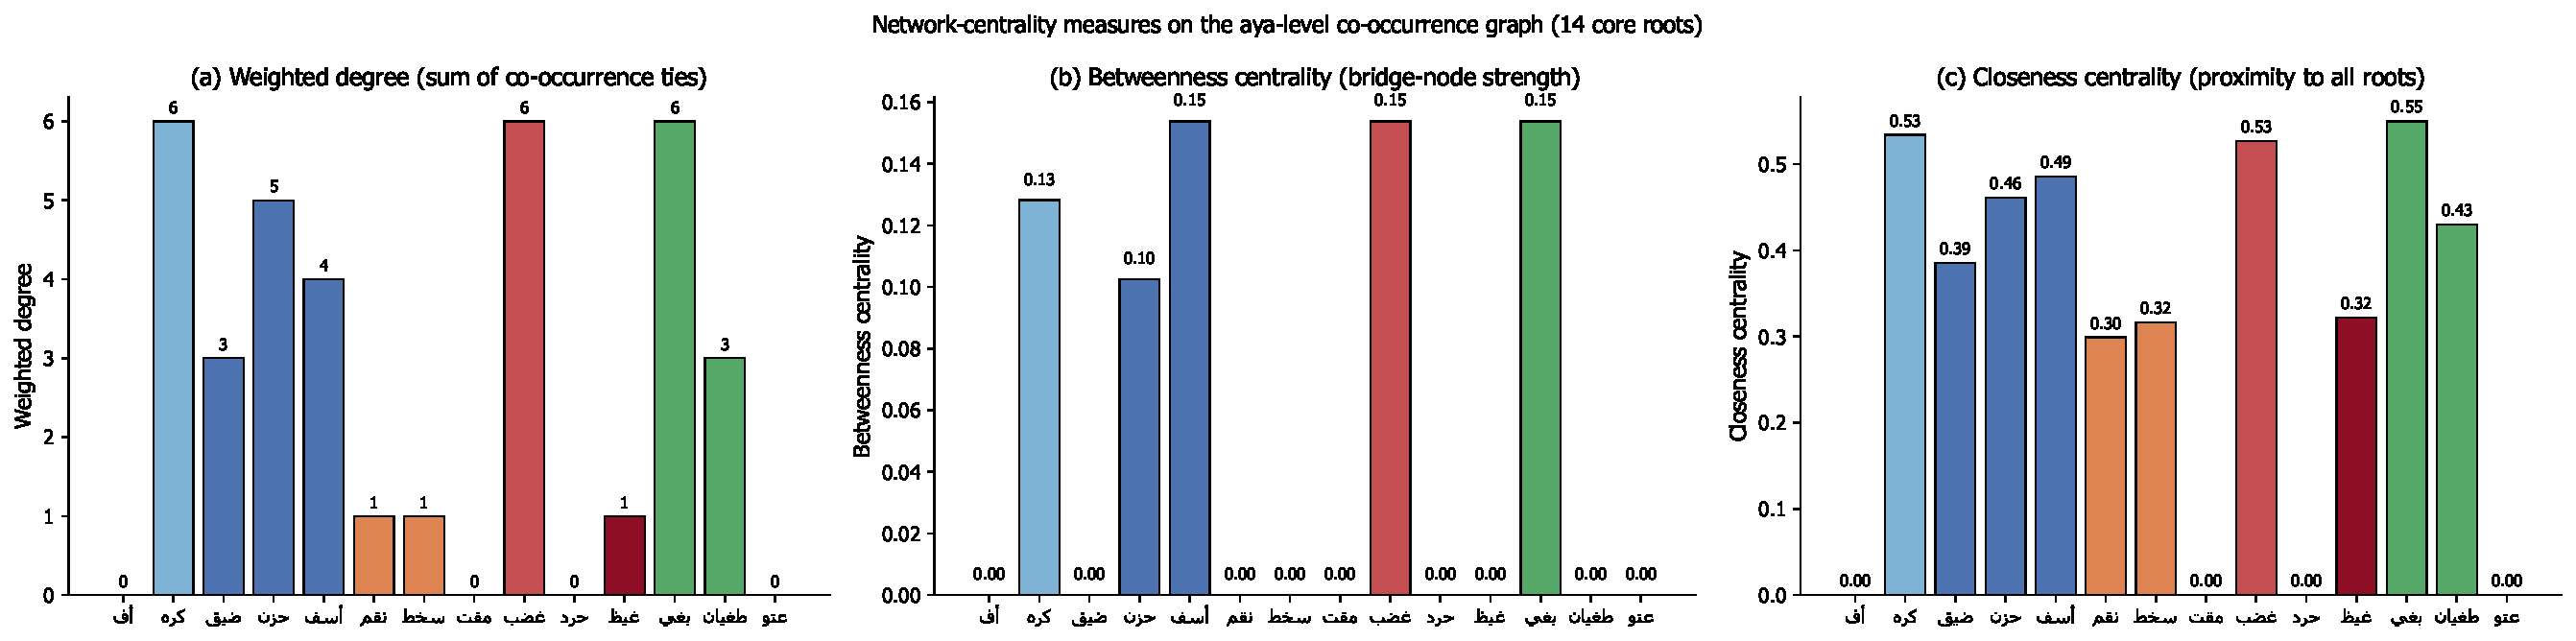
\includegraphics[width=0.95\linewidth,height=\textheight,keepaspectratio]{fig7_centrality.pdf}
\caption{\textbf{Figure 7.} Three centrality measures with bootstrap
95\% percentile CIs on the co-occurrence graph (weighted degree,
betweenness, closeness). \emph{Baghy} leads on closeness (0.55, CI
{[}0.23, 0.84{]}) and shares highest betweenness (0.15, CI {[}0.00,
0.31{]}) with \emph{ghaḍab} and \emph{asaf}. Wide CIs reflect the small
graph; bridging-role claim consistent with point estimates but qualified
by bootstrap (§4.8.2).}
\end{figure}

\subsubsection{4.9. Robustness checks: the umbrella moral
terms}\label{robustness-checks-the-umbrella-moral-terms}

The five umbrella roots (Table 5) confirm that the spectrum's structure
is not artefactual. The opposing patterns of \emph{jrm} (strongly
Meccan) and \emph{fsq} (significantly Medinan) instantiate the same
discursive-contextual specialisation identified for \emph{sakhaṭ} and
\emph{karh} --- the umbrella analysis confirms a general phenomenon.

\textbf{Table 5. Distribution of umbrella moral terms}

\begin{longtable}[]{@{}
  >{\centering\arraybackslash}p{(\linewidth - 10\tabcolsep) * \real{0.2727}}
  >{\centering\arraybackslash}p{(\linewidth - 10\tabcolsep) * \real{0.1364}}
  >{\centering\arraybackslash}p{(\linewidth - 10\tabcolsep) * \real{0.1364}}
  >{\centering\arraybackslash}p{(\linewidth - 10\tabcolsep) * \real{0.1364}}
  >{\centering\arraybackslash}p{(\linewidth - 10\tabcolsep) * \real{0.1364}}
  >{\raggedright\arraybackslash}p{(\linewidth - 10\tabcolsep) * \real{0.1818}}@{}}
\toprule\noalign{}
\begin{minipage}[b]{\linewidth}\centering
Root
\end{minipage} & \begin{minipage}[b]{\linewidth}\centering
n
\end{minipage} & \begin{minipage}[b]{\linewidth}\centering
M
\end{minipage} & \begin{minipage}[b]{\linewidth}\centering
Md
\end{minipage} & \begin{minipage}[b]{\linewidth}\centering
Binomial \emph{p}
\end{minipage} & \begin{minipage}[b]{\linewidth}\raggedright
Interpretation
\end{minipage} \\
\midrule\noalign{}
\endhead
\bottomrule\noalign{}
\endlastfoot
šnʾ & 3 & 1 & 2 & --- & \emph{n} too small \\
jrm & 66 & 60 & 6 & \textless{} 0.0001 & Strongly Meccan;
anti-\emph{shirk} polemic \\
fsq & 54 & 20 & 34 & 0.0007 & Significantly Medinan; community
discipline \\
ẓlm & 315 & 211 & 104 & --- & Pervasive meta-category \\
ʿdw & 106 & 47 & 59 & 0.008 & Tilts Medinan; mutual antagonism \\
\end{longtable}

\subsubsection{4.10. Comparative translation: an illustrative
observation}\label{comparative-translation-an-illustrative-observation}

A four-verse, five-translation sample (Table 6) illustrates the
levelling pattern: \emph{ghayẓ} (Q. 3:134) is rendered with terms
(\emph{anger}, \emph{wrath}, \emph{rage}) routinely used also for
\emph{ghaḍab}, with the containment differentia carried only by the
contextual verb of restraint; \emph{tamayyuz} (Q. 67:8) is rendered
unevenly, with only Arberry's ``well-nigh bursts asunder'' preserving
the structural-disintegration component. The sample is illustrative; a
stratified evaluation across \textasciitilde30 verses with multi-rater
coding is left to future work.

\textbf{Table 6. Translation of four canonical verses across five
English translations} (illustrative sample)

\begin{longtable}[]{@{}
  >{\centering\arraybackslash}p{(\linewidth - 10\tabcolsep) * \real{0.2308}}
  >{\raggedright\arraybackslash}p{(\linewidth - 10\tabcolsep) * \real{0.1538}}
  >{\raggedright\arraybackslash}p{(\linewidth - 10\tabcolsep) * \real{0.1538}}
  >{\raggedright\arraybackslash}p{(\linewidth - 10\tabcolsep) * \real{0.1538}}
  >{\raggedright\arraybackslash}p{(\linewidth - 10\tabcolsep) * \real{0.1538}}
  >{\raggedright\arraybackslash}p{(\linewidth - 10\tabcolsep) * \real{0.1538}}@{}}
\toprule\noalign{}
\begin{minipage}[b]{\linewidth}\centering
Term \& verse
\end{minipage} & \begin{minipage}[b]{\linewidth}\raggedright
Yusuf Ali
\end{minipage} & \begin{minipage}[b]{\linewidth}\raggedright
Pickthall
\end{minipage} & \begin{minipage}[b]{\linewidth}\raggedright
Arberry
\end{minipage} & \begin{minipage}[b]{\linewidth}\raggedright
Saheeh Intl.
\end{minipage} & \begin{minipage}[b]{\linewidth}\raggedright
Hilali-Khan
\end{minipage} \\
\midrule\noalign{}
\endhead
\bottomrule\noalign{}
\endlastfoot
\emph{ḍīq} (Q. 15:97) & ``thy heart is distressed'' & ``thy bosom is at
times oppressed'' & ``thy breast is straitened'' & ``your chest is
constrained'' & ``your breast feels tight'' \\
\emph{ghayẓ} (Q. 3:134) & ``restrain anger'' & ``control their wrath'' &
``restrain their rage'' & ``suppress anger'' & ``repress anger'' \\
\emph{tamayyuz} (Q. 67:8) & ``almost burst with fury'' & ``almost burst
with rage'' & ``well-nigh bursts asunder with fury'' & ``almost bursts
with rage'' & ``almost bursts up with fury'' \\
\emph{ṭughyān} (Q. 96:6) & ``transgresses all bounds'' & ``rebelleth'' &
``waxes insolent'' & ``transgresses'' & ``transgresses (boundary)'' \\
\end{longtable}

\subsubsection{4.11. Summary of computational corroboration
(Supplementary
§S1--S4)}\label{summary-of-computational-corroboration-supplementary-s1s4}

Four NLP analyses extend the main pipeline over the same 312
attestations; full detail at \texttt{paper/english/supplementary.md}.
\textbf{S1 (cross-translation semantic drift)} with multilingual MPNet
over ten parallel renderings recovers three drift bands mapping onto the
spectrum (affective-core lexemes drift \textless{} 0.20,
evaluative-aversion and containment-pressure lexemes \textgreater{}
0.22, \emph{ṭughyān} topping non-hapax) --- convergent with §4.10.
\textbf{S2 (CAMeLBERT-CA clustering)} yields silhouette = −0.082, NMI =
0.077 against the six-stage labelling; a Monte-Carlo baseline (10,000
random 6-partitions of the fourteen roots into stages of the observed
sizes) gives mean random NMI ≈ 0.094 {[}0.041, 0.156{]}. The observed
NMI sits below the random mean --- this is a clear null in which the
model clusters by root identity, and the spectrum adds analytical
structure beyond the language model's distributional view. \textbf{S3
(PMI-weighted network)} corrects raw-count artefacts:
\emph{asaf}--\emph{ghaḍab} (npmi = 0.59) emerges as the strongest signal
and \emph{baghy}'s raw-count dominance is shown to be partly a frequency
artefact. \textbf{S4 (Nöldekean diachronic null)} finds Spearman ρ =
−0.157; R² ≈ 0.025 explains \textless{} 3\% of variance --- a diachronic
effect statistically detectable (\emph{p} = 0.006) but substantively a
null, consistent with the claim that the taxonomy organises by
intensity, not chronology.

\begin{center}\rule{0.5\linewidth}{0.5pt}\end{center}

\subsection{5. Discussion}\label{discussion}

\subsubsection{5.1. The integrated logic of
escalation}\label{the-integrated-logic-of-escalation}

The findings cohere into a single structural claim: the Qur'anic anger
lexicon encodes a logic of escalation along three dimensions --- locus
(inner → outer), intensity (low → high), and scope (individual →
structural). In compact form: \emph{Pre-anger displeasure → Inner
pressure → Evaluative aversion → Active anger → Compressed rage →
Behavioural outcomes (with caveats)}. The arrows index conditional
intensification at each step where regulation may succeed or fail. Stage
6 is distinctive: the move into behavioural outcomes is not a
deterministic escalation from anger but is influenced by independent
vectors (greed, \emph{istikbār}, structural arrogance), which is why the
near-balance between S1--5 and S6 is theoretically informative rather
than paradoxical.

\subsubsection{5.2. Convergence with contemporary emotion
psychology}\label{convergence-with-contemporary-emotion-psychology}

The continuum maps onto four families of contemporary emotion theory at
points of structural convergence, sufficient to ground the
Islamic-psychology implications of §5.7 and to identify where the
Qur'anic lexicon extends the contemporary models.

\textbf{Gross's process model.} Gross (1998, 2014, 2015) partitions
emotion regulation into five sequential strategies (\emph{situation
selection}, \emph{situation modification}, \emph{attentional
deployment}, \emph{cognitive change}, \emph{response modulation}). The
Qur'anic continuum cross-cuts this typology rather than mapping
one-to-one: situation selection is forward-looking and so does not match
the S1 lexemes, which are reactions to a present trigger. \textbf{S1}
(\emph{uff}, \emph{karāha}) is better located at cognitive change /
response-tendency modulation in nuce. \textbf{S2} (\emph{ḍīq},
\emph{ḥuzn}, \emph{asaf}) implicates situation modification and
attentional deployment. \textbf{S3} (\emph{naqm}, \emph{sakhaṭ},
\emph{maqt}) is paradigmatically cognitive change. \textbf{S4}
(\emph{ghaḍab}, \emph{ḥard}) lies at the response-selection threshold.
\textbf{S5} is response modulation with two sub-strategies: \emph{kaẓm}
(Q. 3:134) is closest to \emph{expressive suppression}, but the Qur'anic
moral commendation of \emph{kāẓimīn al-ghayẓ} need not entail the
physiological costs Gross associates with suppression, and Sufi readings
(al-Qushayrī's \emph{Laṭāʾif al-Ishārāt} ad loc.) tilt the construct
toward \emph{cognitive reappraisal} in the \emph{taqwā} frame; we do not
read \emph{kāẓim al-ghayẓ} as unambiguously expressive-suppression.
\emph{Tamayyuz} figures the failure mode regardless. \textbf{S6} lies
beyond the episode-bounded scope of Gross's model --- structural-moral
pathologies of personhood, with the §4.8.5 bidirectional-causation
caveat.

\textbf{Plutchik; Spielberger.} Plutchik's (1980, 2001) three-level
escalation (annoyance → anger → rage) is refined by the Qur'anic
continuum, which partitions annoyance into vocal irritation (\emph{uff},
S1), inner aversion (\emph{karāha}, S1), and inner pressure (S2) ---
three stages where Plutchik has one label --- and inserts compressed
rage (\emph{ghayẓ}, S5) between anger (≈ S4 \emph{ghaḍab}) and terminal
rage. Spielberger's STAXI-2 (1999) trichotomy of \emph{trait},
\emph{state}, and \emph{control} is realised at the lexical surface:
trait-like sustained states (\emph{ḥuzn}, \emph{ḍīq}, \emph{karāha});
state-like situational responses (\emph{sakhaṭ}, \emph{maqt},
\emph{ghaḍab}); and \emph{kaẓm} (Q. 3:134) as the Qur'anic anger-control
lexeme, operationally close to Spielberger's anger-in / suppression
construct but with explicit moral commendation.

\textbf{Appraisal theory: Scherer's checks and Roseman's
\emph{ṭughyān}-pattern.} Appraisal theory (Frijda 1986; Lazarus 1991;
Scherer 2001, 2005; Roseman 1996) holds that emotional response is
determined not by stimulus alone but by cognitive \emph{appraisal} along
defined dimensions. Scherer's component-process model specifies four
sequential checks; the Stage-3 lexemes operate as a lexicon for the
normative-significance check at progressively higher intensities
(\emph{naqm} → \emph{sakhaṭ} → \emph{maqt}). Sūrat al-ʿAlaq (Q. 96:6--7)
conditions \emph{ṭughyān} on the appraisal of \emph{istighnāʾ}: the
agent perceives high coping potential, low external constraint, and
self-agency. On Roseman's (1996) appraisal structure, defiance and
contempt are \emph{other-caused} and \emph{motive-inconsistent} (the
agent rebels against an other-imposed normative constraint perceived as
inconsistent with the agent's self-conception). \emph{Ṭughyān} on
\emph{istighnāʾ} fits this pattern: the divine command is the
other-caused, motive-inconsistent constraint that \emph{istighnāʾ}
construes as dispensable. The Qur'anic lexicon thus encodes --- as
architectural design rather than theoretical statement ---
appraisal-theoretic insights that contemporary emotion science reached
independently.

\subsubsection{5.3. The phenomenology/outcomes
balance}\label{the-phenomenologyoutcomes-balance}

A naive ten-root reading once suggested 2.4× more attestations at the
behavioural pole than at S1--3 combined. The revised fourteen-root
inventory (167 / 145) corrects that picture: the expanded
phenomenological vocabulary brings the lower stages into balance with
Stage 6, consistent with both a richer affective lexicon and the
bidirectional causal relation between Stage-6 lexemes and anger. In
Fauconnier and Turner's (2002: 17--57) terms, Stage 6 operates as a
conceptual blend whose input spaces are wrong-doing-as-supremacism and
anger-as-pressure.

\subsubsection{5.4. Discursive-contextual specialisation and Cultural
Linguistics}\label{discursive-contextual-specialisation-and-cultural-linguistics}

The FDR-surviving tilts of \emph{karh} (Medinan), \emph{baghy} (Meccan),
\emph{ghayẓ} (Medinan), the borderline \emph{sakhaṭ} (Medinan), the
contextual Meccan tilts of \emph{asaf}, \emph{naqm}, and \emph{ʿutuww},
and the umbrella patterns \emph{jrm} (Meccan) / \emph{fsq} (Medinan)
together instantiate \emph{discursive-contextual specialisation} ---
members of multi-lexeme fields attaching to specific discursive
registers. The attachments are non-random: \emph{sakhaṭ} to the
\emph{Munāfiqūn} (a Medinan phenomenon), \emph{karh} to the structural
\emph{ikrāh} idiom of Medinan community discipline, \emph{ghayẓ} to the
\emph{kaẓm} pedagogy of Medinan ethics, \emph{asaf} to prior-prophet
narratives (Meccan-rhetorical), \emph{jrm} to anti-\emph{shirk} polemic
(Meccan), \emph{fsq} to intra-community discipline (Medinan). El-Awa
(2006) and Sinai (2017, 2023) supply the framework: specialisation is
the pattern one expects from the Qur'an's gradual response to evolving
sociolinguistic contexts.

Read through Sharifian (2011), the same data illuminate the
universal--culturally-elaborated distinction of §2.3.2: the primary
metaphors (ANGER IS HEAT; EMOTIONAL CONTAINMENT IS PHYSICAL CONTAINMENT)
are robustly attested in the Qur'anic \emph{ghayẓ}--\emph{kaẓm} register
and support the CMT universalist claim; the \emph{culturally elaborated}
layer --- the distribution of affect across \emph{qalb} (S2 \emph{ḍīq
al-ṣadr}), \emph{ṣadr} (S2), and \emph{nafs} (S2 \emph{asaf al-nafs}),
the moral commendation of \emph{kaẓm} in the \emph{taqwā} frame, the
\emph{Munāfiqūn}-attachment of \emph{sakhaṭ}, and the \emph{tamayyuz}
construal of Q. 67:8 --- is what the Qur'anic data illuminate beyond the
universalist baseline.

\subsubsection{5.5. Q. 67:8 and the container metaphor: a focused
comparative
survey}\label{q.-678-and-the-container-metaphor-a-focused-comparative-survey}

The Qur'anic \emph{ghayẓ--kaẓm--tamayyuz} triad maps onto stages
(2)--(4) of the Lakoff--Kövecses scenario with unusual lexical
transparency at stage (4): English exemplars (\emph{blew his top})
lexicalise the failure-mode as \emph{exit of contents} with the
container preserved, whereas Q. 67:8, under the complex container
metaphor of §2.3.1, supports the construal of vessel-internal failure
(§4.7.2). A six-tradition survey contextualises the claim.
\emph{Akkadian}: \emph{libbu} and \emph{kabattu} as filled containers
(CAD L 163--164; Bodi 2018; Neo-Assyrian bodily-mapping work in Lauri et
al.~2024 confirms the FILLING/HEAT-IN-CONTAINER schema). \emph{Biblical
Hebrew}: \emph{ḥēmâ} and \emph{ḥarôn-ʾaph} (Kruger 2000, 2015) both
EXIT-typed --- except Job 32:19 (\emph{kĕ-yayin lōʾ-yippātēaḥ \ldots{}
yibbāqēaʿ}), where \emph{bāqaʿ} names the structural failure of the
vessel; this is the one clear pre-Qur'anic Northwest-Semitic precedent.
\emph{Homeric Greek}: \emph{kholos} and \emph{mēnis} in fluid-and-heat
schemas with no Iliadic vessel-rupture (Muellner 1996; Cairns 2003).
\emph{Vedic and Classical Sanskrit}: \emph{krodha} and \emph{manyu} in
FIRE and WEAPON-RELEASE schemas, not vessel-disintegration.
\emph{Classical and Modern Chinese}: \emph{nù}, \emph{fèn}, \emph{qì}
with HOT \emph{QÌ} IN A CONTAINER (Yu 1995; Kövecses, Benczes and Szelid
2025). \emph{Pre-Islamic Jāhilī Arabic}: \emph{ḥamiya} and \emph{ghalā}
alongside \emph{ghayẓ} in the cognate fluid-heat register
(cf.~\emph{al-Mufaḍḍaliyyāt} nos. 38, 87, ʿAntara's \emph{Muʿallaqa} ll.
32--35; Webb 2016: 213--245). Five of the six traditions concentrate on
filling, heating, exit/overflow; the Hebrew Bible alone offers a clear
parallel to vessel-rupture proper. We hold our claim at ``an early and
unusually transparent'' lexicalisation, with Job 32:19 acknowledged as a
structurally cognate Northwest-Semitic precedent. The Qur'anic data
strengthen the universalist hypothesis of CMT and extend the empirical
base to seventh-century Arabic.

\begin{figure}
\centering
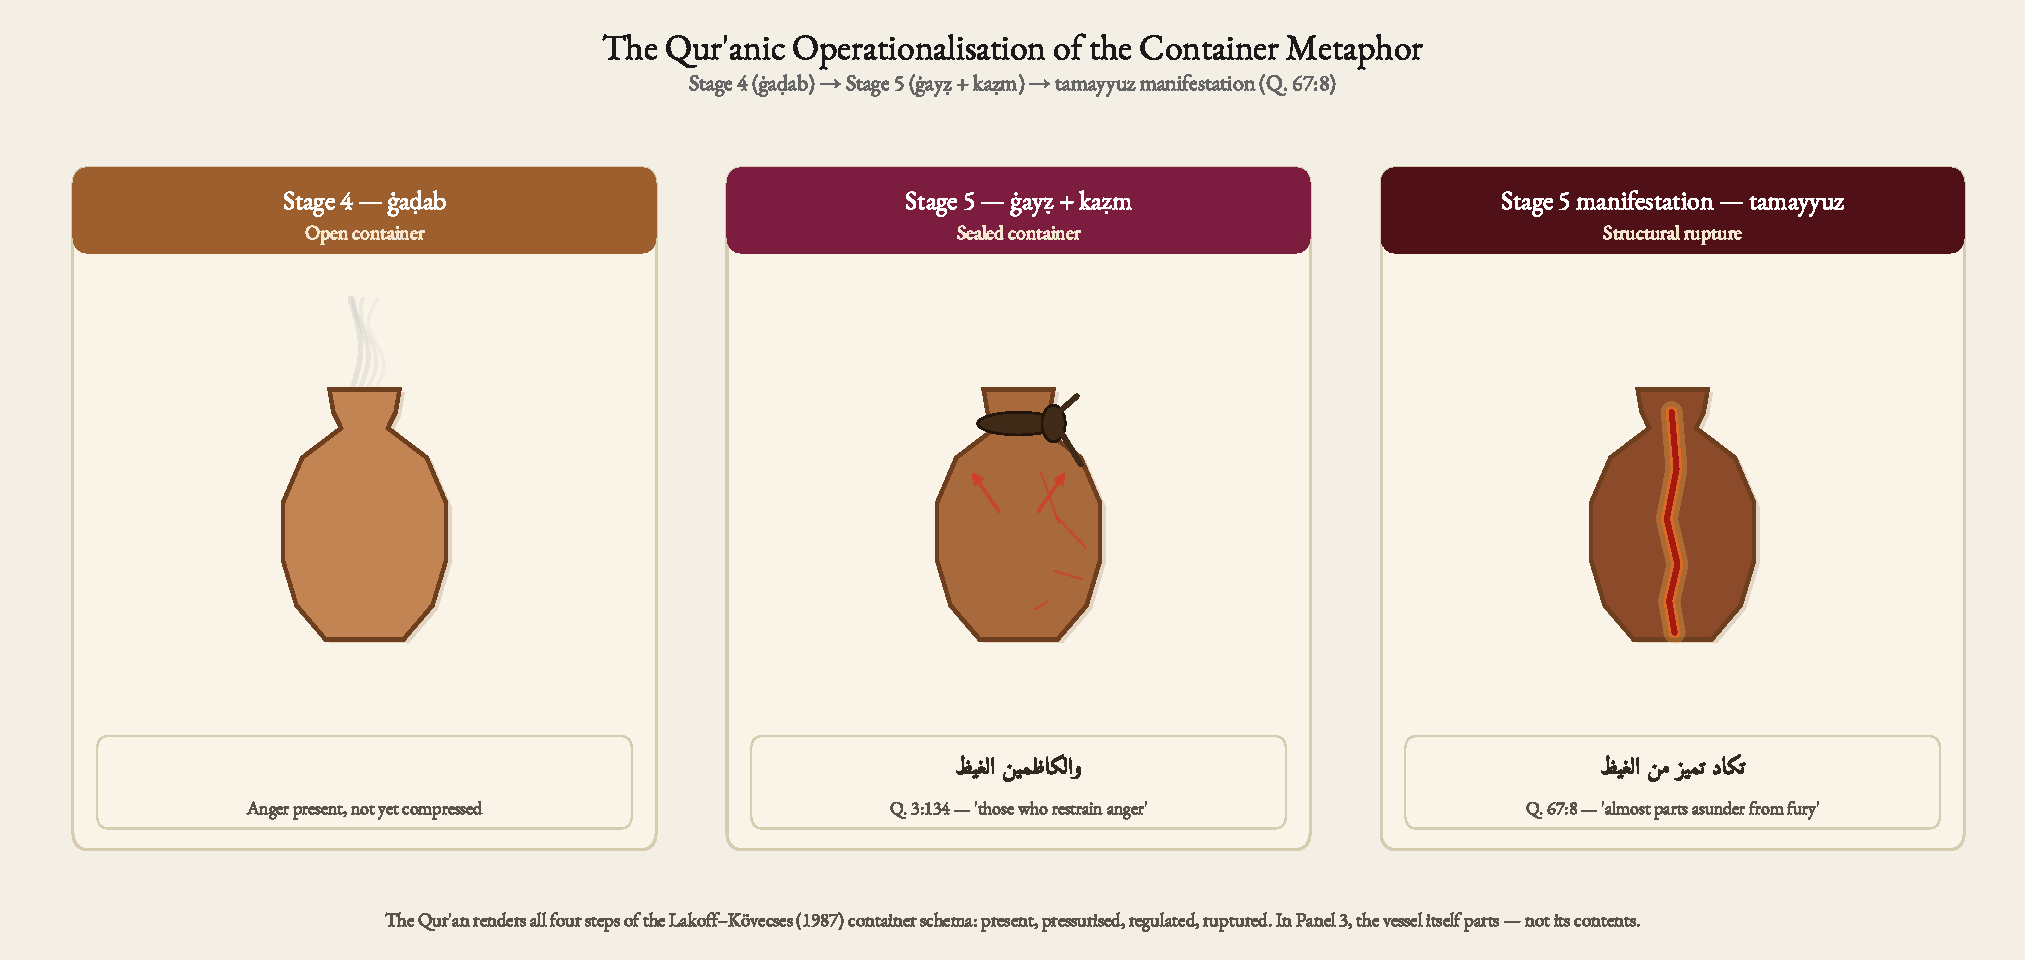
\includegraphics[width=1\linewidth,height=\textheight,keepaspectratio]{fig6_metaphor_v2.pdf}
\caption{\textbf{Figure 6.} \emph{Illustrative} schematisation of the
ANGER-IS-A-PRESSURIZED-CONTAINER complex metaphor (after Lakoff and
Kövecses 1987), instantiated by \emph{ghaḍab → ghayẓ + kaẓm → tamayyuz}.
Panel 1 (S4): \emph{ghaḍab} --- open container, affect dissipating into
language. Panel 2 (S5, Q. 3:134): \emph{ghayẓ} sealed by \emph{kaẓm}.
Panel 3 (S5 manifestation, Q. 67:8): \emph{tamayyuz} --- the construal
of constituent-separation as vessel-internal failure (§4.7.2). The
figure is heuristic; evidence is borne by the lexicographic and
exegetical analysis of §4.7 and §5.5.}
\end{figure}

\subsubsection{5.6. Implications for Qur'anic
translation}\label{implications-for-quranic-translation}

A graded reference model of the spectrum offers a principled corrective
to the levelling pattern that Gaanoun and Alsuhaibani (2025) and Khan et
al.~(2025) document at the sentiment-category level. We do not, on the
strength of the four-verse illustrative sample of §4.10, advance
translation prescriptions; a systematic stratified evaluation
(\textasciitilde30 verses across the six stages, multi-rater coded
against the spectrum) is the prerequisite. Candidate equivalents for
each spectrum lexeme are catalogued in the project repository for use by
translators wishing to mark intensity-position lexically.

\subsubsection{5.7. Implications for Islamic
psychology}\label{implications-for-islamic-psychology}

The continuum offers a culturally-grounded framework mapping onto
Gross's model without importing secular vocabulary, with three
conceptual implications: (i) \emph{Prevention} --- early-stage
recognition through the indigenous S1--2 lexicon supports CBT-style
interception of affective dysregulation; (ii) \emph{Crisis intervention}
--- \emph{kaẓm} integrates with contemporary suppression-and-reappraisal
techniques; (iii) \emph{Rehabilitation} --- post-failure Stage 6 is
framed as recoverable through \emph{tawba}. These are conceptual; their
translation into validated clinical interventions awaits empirical
studies.

\begin{center}\rule{0.5\linewidth}{0.5pt}\end{center}

\subsection{6. Conclusion}\label{conclusion}

\subsubsection{6.1. Substantive
contributions}\label{substantive-contributions}

\emph{Methodologically}, the integration of Izutsu's semantic-field
analysis, Kennedy--Sassoon scalar semantics, and Lakoff--Kövecses CMT
--- coupled with a reproducible computational pipeline over the QAC ---
produces an apparatus stronger than the sum of its parts; to our
knowledge, this trifold integration with corpus-empirical validation has
not been deployed in Qur'anic studies, although Qāʾimīniyā (2011, 2014)
and Pakatchi and Afrashi (2020) have integrated Izutsu and CMT.

\emph{Descriptively}, we produce a reproducible concordance of 312
attestations with FDR-adjusted binomial tests, marginal-preserving
permutation null \emph{p}-values, and bootstrap 95\% CIs on every
centrality estimate.

\emph{Theoretically}, we formulate and defend the \emph{Qur'anic
Action-Intensity Continuum Hypothesis}: the fourteen lexemes operate as
a single graded continuum structured by intensity of action and
partitioned into six stages, supported by qualitative evidence from the
four authoritative lexica and the broadened \emph{tafsīr} consultation,
and by quantitative evidence from frequency, distribution, morphology,
and network structure. The κ = 0.79-validated audit grounds the
bidirectional-causation reading of Stage 6; the six-tradition survey of
§5.5 calibrates Q. 67:8 as an early and unusually transparent --- rather
than uniquely transparent --- exemplification of vessel-internal
failure, with Job 32:19 (\emph{bāqaʿ}) acknowledged as a structurally
cognate Northwest-Semitic precedent.

\subsubsection{6.2. Answers to the research
questions}\label{answers-to-the-research-questions}

\textbf{RQ1--RQ2.} The anger-spectrum field is a fourteen-node lexical
network organised by intensity of action; \emph{baghy} is the bridge
node (closeness 0.55; \textasciitilde53\% of cross-field ties to the
umbrella moral-evaluation terms); stage-internal hubs are \emph{ḥuzn}
(S2) and \emph{ghaḍab} (S4). \textbf{RQ3.} The empirical distribution is
\emph{consistent with} the continuum: asymptotic χ²(5) = 227.15 large,
permutation null \emph{p} = 0.24; S1--5/S6 χ²(1) = 1.55 fails to reject,
consistent with the bidirectional-causation reading supported by the κ =
0.79 audit (A = 26\%, S = 49\%, A+S = 25\%; A-only re-analysis χ²(1) =
81.4, \emph{p} \textless{} 0.001). Three roots survive Holm-Bonferroni
emphatically (\emph{karh}, \emph{baghy}, \emph{ghayẓ}); \emph{sakhaṭ}
sits at adj. \emph{p} = 0.050. \textbf{RQ4.} The continuum is
structurally homologous with Gross (S1--5), Plutchik, Spielberger, and
Lazarus--Scherer--Roseman appraisal theory (sūrat al-ʿAlaq, Q. 96:6--7,
\emph{ṭughyān} on \emph{istighnāʾ}); it extends beyond all four at Stage
6. \textbf{RQ5.} Conditional implications follow for Qur'anic
translation (§5.6) and Islamic psychology (§5.7).

\subsubsection{6.3. Limitations and future
work}\label{limitations-and-future-work}

Five limitations point to constructive next steps. (i)
\emph{Surface-lexical scope}: discourse-analytic close-reading of the
spectrum's narrative deployment across suras is left for future work.
(ii) \emph{Tafsīr engagement}: a deep-dive indexing the full
classical/medieval/Sufi/modernist tradition with κ-validated multi-coder
reading on contested verses would deepen exegetical grounding. (iii)
\emph{Cognitive-linguistic apparatus}: engagement with classical
\emph{bayān} theory (al-Jurjānī, al-Sakkākī) would supply an indigenous
substrate. (iv) \emph{Ḥadīth integration}: a parallel concordance over
Ṣaḥīḥ al-Bukhārī, Ṣaḥīḥ Muslim, and al-Kāfī would supply convergent
evidence on \emph{kaẓm} and a replication test for the underpowered
\emph{asaf} distribution. (v) \emph{Islamic-psychology
operationalisation}: §5.7's implications await pilot studies of
\emph{kaẓm}-grounded emotion-regulation training, validated against the
STAXI and DERS. Computational evidence remains a complement to, not a
replacement for, the classical philological and exegetical tradition.

\subsubsection{6.4. Closing remark}\label{closing-remark}

The Qur'anic lexicon encodes a sophisticated theory of the anger
spectrum in the architecture of its semantic surface. Recovering it
requires the integration of classical philological attentiveness,
contemporary linguistic-theoretical precision, and corpus-computational
verifiability.

\begin{center}\rule{0.5\linewidth}{0.5pt}\end{center}

\subsection{Acknowledgements}\label{acknowledgements}

The authors thank Kais Dukes (in memoriam) and the team behind the
Quranic Arabic Corpus, and the Tanzil Project, for releasing the
morphological and textual resources without which this kind of empirical
Qur'anic analysis would not be feasible. We thank Urmia University for
institutional support.

\subsection{Funding}\label{funding}

This research received no specific grant from any funding agency in the
public, commercial, or not-for-profit sectors.

\subsection{Competing interests}\label{competing-interests}

The authors declare no competing financial or non-financial interests.

\subsection{Author note: parallel-language
submission}\label{author-note-parallel-language-submission}

An independent Persian-language paper using the same corpus dataset is
concurrently under consideration at \emph{Pizhūhish-hā-yi
Zabānshinākhtī-yi Qurʾān}. The two papers do not share content or cite
each other; the empirical pipeline is the only shared element, and each
paper presents an independent argument for its own scholarly audience.

\subsection{Ethics statement}\label{ethics-statement}

This study uses only publicly-released text-corpus data (the Quranic
Arabic Corpus, GPL-licensed; the Tanzil Quran text, CC-BY-ND 3.0). No
human or animal subjects were involved at any stage. As a corpus-only
philological-computational analysis, the work is exempt from
human-subjects review under the standards of Urmia University and of
comparable institutions.

\subsection{Author contributions}\label{author-contributions}

K.J. (corresponding author) conceived the project, developed the
theoretical framework, conducted the lexicographic and
\emph{tafsīr}-tradition analysis, drafted the manuscript, and is
responsible for the final form of the argument. A.J. contributed to the
theoretical framework, the design of the computational pipeline, and
editorial revision. Both authors approved the final manuscript and are
jointly accountable for its content.

\subsection{Author affiliations}\label{author-affiliations}

\textbf{Karim Jabbary} (corresponding author). Department of Arabic
Language and Literature, Faculty of Literature and Humanities, Urmia
University, Urmia, Iran. \emph{email:} k.jabbary@urmia.ac.ir.

\textbf{Ali Jabbary}. Faculty of Computer Engineering, Urmia University,
Urmia, Iran. \emph{email:} a.jabbary@urmia.ac.ir.

\subsection{Data and Code
Availability}\label{data-and-code-availability}

All code, data, concordance CSV outputs, and figure-generation scripts
are released open-source at:

\begin{quote}
\href{https://github.com/ali-kin4/quranic-emotion-spectrum}{github.com/ali-kin4/quranic-emotion-spectrum}
\end{quote}

The repository contains: (i) the Python pipeline under MIT License; (ii)
the Quranic Arabic Corpus (Dukes 2011) under its original GPL; (iii) the
complete CSV concordance for the fourteen core spectrum roots (312
attestations), distributional summaries, statistical tests,
network-centrality outputs, and umbrella-cooccurrence tables; (iv) PDF
and PNG versions of the figures published with this paper and with the
Supplementary Material; (v) the SHA-256 hash of the QAC v0.4 source file
and the manual-validation audit. The four statistical analyses of
§§4.2--4.9 can be regenerated end-to-end by:

\begin{Shaded}
\begin{Highlighting}[]
\ExtensionTok{pip}\NormalTok{ install }\AttributeTok{{-}r}\NormalTok{ analysis/requirements.txt}
\ExtensionTok{python}\NormalTok{ analysis/extract\_concordance.py}
\ExtensionTok{python}\NormalTok{ analysis/advanced\_metrics.py}
\ExtensionTok{python}\NormalTok{ analysis/visualize\_spectrum.py}
\ExtensionTok{python}\NormalTok{ analysis/visualize\_advanced.py}
\end{Highlighting}
\end{Shaded}

The four computational corroboration analyses reported in Supplementary
Material S1--S4 are produced by \texttt{nlp\_upgrade\_colab.py}, which
requires a CUDA-enabled GPU for the multilingual-MPNet and CAMeLBERT-CA
inference. A Colab notebook is available in the repository with pinned
model snapshots and an expected runtime of \textasciitilde25 minutes on
a T4 GPU; CSV outputs are committed under \texttt{outputs/nlp\_upgrade/}
so that reviewers can inspect the numerical results without re-running
the GPU pipeline.

\begin{center}\rule{0.5\linewidth}{0.5pt}\end{center}

\subsection{Bibliography}\label{bibliography}

References use Harvard author-date in-text citation; the Bibliography is
unified and alphabetised by author surname (the Arabic article
\emph{al-} is ignored for alphabetisation, sorting on the
post-\emph{al-} letter). Persian-language and classical-Arabic entries
are interleaved in the single sequence.

Agresti, A. (2013) \emph{Categorical Data Analysis}, 3rd edn, Hoboken,
NJ: John Wiley \& Sons.

Akra, D., Hammouda, T. and Jarrar, M. (2025) \emph{QuranMorph:
Morphologically Annotated Quranic Corpus}, arXiv preprint 2506.18148,
https://arxiv.org/abs/2506.18148.

Albayrak, I. (2020) `Semantics of the Qurʾānic Weltanschauung: A
Critical Analysis of Toshihiko Izutsu's Works', \emph{American Journal
of Islam and Society} 37(1--2).

Averill, J. R. (1982) \emph{Anger and Aggression: An Essay on Emotion},
New York: Springer-Verlag.

Berkowitz, L. (1993) \emph{Aggression: Its Causes, Consequences, and
Control}, New York: McGraw-Hill.

Bodi, D. (2018) `An Akkadian-Aramaic Idiomatic Expression in Ezekiel
16:30 \emph{amūlâ libbātēk} ``I am filled with anger against you'', and
Remarks on the Languages in Persian Times', \emph{Transeuphratène} 50,
pp.~13--38.

Cairns, D. L. (2003) `Ethics, Ethology, Terminology: Iliadic Anger and
the Cross-cultural Study of Emotion', in S. Braund and G. W. Most (eds),
\emph{Ancient Anger: Perspectives from Homer to Galen}, Yale Classical
Studies 32, Cambridge: Cambridge University Press, pp.~11--49.

\emph{Chicago Assyrian Dictionary (CAD)} (1956--2010), ed.~M. T. Roth et
al., 21 vols, Chicago: The Oriental Institute.

Cochran, W. G. (1954) `Some Methods for Strengthening the Common χ²
Tests', \emph{Biometrics} 10(4), pp.~417--451.

Derki, M. (2022) `Conceptualization of Anger in Modern Standard Arabic
and English: A Comparative Study', \emph{Professional Discourse and
Communication}.

Dukes, K. (2011) \emph{Quranic Arabic Corpus (Morphology, Version 0.4)},
Leeds: University of Leeds, https://corpus.quran.com.

El-Awa, S. M. S. (2006) \emph{Textual Relations in the Qurʾan:
Relevance, Coherence and Structure}, Routledge Studies in the Qurʾan,
London and New York: Routledge.

al-Fīrūzābādī, Muḥammad. \emph{al-Qāmūs al-Muḥīṭ}, Beirut: Muʾassasat
al-Risālah.

Fauconnier, G. and Turner, M. (2002) \emph{The Way We Think: Conceptual
Blending and the Mind's Hidden Complexities}, New York: Basic Books.

Fisher, R. A. (1922) `On the Interpretation of χ² from Contingency
Tables, and the Calculation of \emph{P}', \emph{Journal of the Royal
Statistical Society} 85(1), pp.~87--94.

Frijda, N. H. (1986) \emph{The Emotions}, Studies in Emotion and Social
Interaction, Cambridge and Paris: Cambridge University Press and
Éditions de la Maison des Sciences de l'Homme.

Gaanoun, K. and Alsuhaibani, M. (2025) `Sentiment Preservation in Quran
Translation with Artificial Intelligence Approach: Study in Reputable
English Translation of the Quran', \emph{Humanities and Social Sciences
Communications} 12(1), DOI: 10.1057/s41599-024-04181-0.

Gross, J. J. (1998) `The Emerging Field of Emotion Regulation: An
Integrative Review', \emph{Review of General Psychology} 2(3),
pp.~271--299.

Gross, J. J. (ed.) (2014) \emph{Handbook of Emotion Regulation}, 2nd
edn, New York: Guilford Press.

Gross, J. J. (2015) `Emotion Regulation: Current Status and Future
Prospects', \emph{Psychological Inquiry} 26(1), pp.~1--26.

Grady, J. E. (1997) \emph{Foundations of Meaning: Primary Metaphors and
Primary Scenes}, PhD dissertation, University of California, Berkeley.

Ibn ʿĀshūr, Muḥammad al-Ṭāhir (1984) \emph{al-Taḥrīr wa-l-Tanwīr},
Tunis: al-Dār al-Tūnisiyyah li-l-Nashr.

Ibn Fāris, Aḥmad (1979) \emph{Muʿjam Maqāyīs al-Lughah}, ed.~ʿA. M.
Hārūn, Beirut: Dār al-Fikr.

Ibn Kathīr, Ismāʿīl (1999) \emph{Tafsīr al-Qurʾān al-ʿAẓīm}, ed.~S.
al-Salāmah, 8 vols, Riyadh: Dār Ṭaybah.

Ibn Manẓūr, Muḥammad (1993) \emph{Lisān al-ʿArab}, 3rd edn, Beirut: Dār
Ṣādir.

Izutsu, T. (1959) \emph{The Structure of the Ethical Terms in the Koran:
A Study in Semantics}, Studies in the Humanities and Social Relations 2,
Tokyo: Keio Institute of Philological Studies.

Izutsu, T. (1964) \emph{God and Man in the Koran: Semantics of the
Koranic Weltanschauung}, Tokyo: Keio Institute of Cultural and
Linguistic Studies.

Izutsu, T. (2002) \emph{Ethico-Religious Concepts in the Qurʾān}, rev.
edn, Montreal: McGill-Queen's University Press (orig. 1966).

Jamison, S. W. and Brereton, J. P. (2014) \emph{The Rigveda: The
Earliest Religious Poetry of India}, 3 vols, New York: Oxford University
Press.

Kassinove, H. and Tafrate, R. C. (2002) \emph{Anger Management: The
Complete Treatment Guidebook for Practitioners}, Atascadero, CA: Impact
Publishers.

Kennedy, C. (1999) \emph{Projecting the Adjective: The Syntax and
Semantics of Gradability and Comparison}, Outstanding Dissertations in
Linguistics, New York: Garland.

Kennedy, C. (2007) `Vagueness and Grammar: The Semantics of Relative and
Absolute Gradable Adjectives', \emph{Linguistics and Philosophy} 30(1),
pp.~1--45.

Khan, M. T. et al.~(2025) `A Literature Review on Natural Language
Processing Techniques for Qurʾānic Studies: Challenges and Insights',
\emph{Frontiers in Signal Processing} 5, 1535166, DOI:
10.3389/frsip.2025.1535166.

Kövecses, Z. (1986) \emph{Metaphors of Anger, Pride, and Love: A Lexical
Approach to the Structure of Concepts}, Pragmatics \& Beyond VII:8,
Amsterdam: John Benjamins.

Kövecses, Z. (2000) \emph{Metaphor and Emotion: Language, Culture, and
Body in Human Feeling}, Cambridge: Cambridge University Press.

Kövecses, Z. (2010) \emph{Metaphor: A Practical Introduction}, 2nd edn,
Oxford: Oxford University Press.

Kövecses, Z. (2020) \emph{Extended Conceptual Metaphor Theory},
Cambridge: Cambridge University Press.

Kövecses, Z., Benczes, R. and Szelid, V. (eds) (2025) \emph{Metaphors of
ANGER across Languages: Universality and Variation}, 2 vols, Comparative
Handbooks of Linguistics 8, Berlin and Boston: De Gruyter Mouton.

Kruger, P. A. (2000) `A Cognitive Interpretation of the Emotion of Anger
in the Hebrew Bible', \emph{Journal of Northwest Semitic Languages}
26(1), pp.~181--193.

Kruger, P. A. (2015) `Emotions in the Hebrew Bible: A Few Observations
on Prospects and Challenges', \emph{Old Testament Essays} 28(2),
pp.~395--420.

Lakoff, G. and Johnson, M. (1980) \emph{Metaphors We Live By}, Chicago:
University of Chicago Press.

Lakoff, G. and Kövecses, Z. (1987) `The Cognitive Model of Anger
Inherent in American English', in D. Holland and N. Quinn (eds),
\emph{Cultural Models in Language and Thought}, Cambridge: Cambridge
University Press, pp.~195--221.

Landis, J. R. and Koch, G. G. (1977) `The Measurement of Observer
Agreement for Categorical Data', \emph{Biometrics} 33(1), pp.~159--174.

Lauri, J., Svärd, S., Alstola, T., Jauhiainen, H., Sahala, A., Lindén,
K., Sams, M. and Nummenmaa, L. (2024) `Embodied Emotions in Ancient
Neo-Assyrian Texts Revealed by Bodily Mapping of Emotional Semantics',
\emph{iScience} 27(12), 111365.

Lazarus, R. S. (1991) \emph{Emotion and Adaptation}, New York: Oxford
University Press.

Maalej, Z. (2004) `Figurative Language in Anger Expressions in Tunisian
Arabic: An Extended View of Embodiment', \emph{Metaphor and Symbol}
19(1), pp.~51--75.

Maalej, Z. (2007) `The Embodiment of Fear Expressions in Tunisian
Arabic: Theoretical and Practical Implications', in F. Sharifian and G.
B. Palmer (eds), \emph{Applied Cultural Linguistics: Implications for
Second Language Learning and Intercultural Communication}, Converging
Evidence in Language and Communication Research 7, Amsterdam: John
Benjamins, pp.~87--104.

Maalej, Z. A. and Yu, N. (eds) (2011) \emph{Embodiment via Body Parts:
Studies from Various Languages and Cultures}, Human Cognitive Processing
31, Amsterdam and Philadelphia: John Benjamins.

Marcus-Newhall, A., Pedersen, W. C., Carlson, M. and Miller, N. (2000)
`Displaced Aggression is Alive and Well: A Meta-analytic Review',
\emph{Journal of Personality and Social Psychology} 78(4), pp.~670--689.

Mehta, C. R. and Patel, N. R. (1983) `A Network Algorithm for Performing
Fisher's Exact Test in \emph{r} × \emph{c} Contingency Tables',
\emph{Journal of the American Statistical Association} 78(382),
pp.~427--434.

al-Mostafawī, Ḥasan (1995) \emph{al-Taḥqīq fī Kalimāt al-Qurʾān
al-Karīm}, 14 vols, Tehran: Wizārat al-Thaqāfah wa-l-Irshād al-Islāmī.

Mottaghi, M. S. et al.~(2024) `A Graph-based Algorithm for Clustering
Qurʾānic Surahs', \emph{Signal and Data Processing Journal (Iran)}.

Muellner, L. C. (1996) \emph{The Anger of Achilles: Mēnis in Greek
Epic}, Ithaca, NY: Cornell University Press.

Nandan, M., Godbole, I., Kapparad, P. and Bhattacharjee, S. (2025)
`Comparative Analysis of Religious Texts: NLP Approaches to the Bible,
Quran, and Bhagavad Gītā', in \emph{Proceedings of the Workshop on New
Horizons in Computational Linguistics for Religious Texts (CLRel)},
Stroudsburg, PA: Association for Computational Linguistics.

Narimani, Z., Iqbali, M. and Chari, M. (2021) `Semantic Re-analysis of
the Words \emph{ghayẓ}, \emph{ghaḍab}, and \emph{sakhaṭ} in the Holy
Qurʾān with an Exegetical Approach' {[}in Persian{]},
\emph{Pizhūhish-hā-yi Qurʾān va Ḥadīth} (University of Tehran) 54(1),
pp.~219--239.

Neuwirth, A. (2019) \emph{The Qur'an and Late Antiquity: A Shared
Heritage}, trans. S. Wilder, Oxford: Oxford University Press.

Pakatchi, A. and Afrashi, A. (2020) \emph{Rūykardhā-yi Maʿnā-shinākhtī
dar Muṭālaʿāt-i Qurʾānī} {[}Semantic Approaches in Qurʾānic Studies; in
Persian{]}, Tehran: Pizhūhishgāh-i ʿUlūm-i Insānī va Muṭālaʿāt-i
Farhangī.

Patefield, W. M. (1981) `Algorithm AS 159: An Efficient Method of
Generating Random \emph{R} × \emph{C} Tables with Given Row and Column
Totals', \emph{Journal of the Royal Statistical Society, Series C
(Applied Statistics)} 30(1), pp.~91--97.

Plutchik, R. (1980) \emph{Emotion: A Psychoevolutionary Synthesis}, New
York: Harper \& Row.

Plutchik, R. (2001) `The Nature of Emotions', \emph{American Scientist}
89(4), pp.~344--350.

Qāʾimīniyā, ʿA. (2011) \emph{Maʿnāshināsī-yi Shinākhtī-yi Qurʾān}
{[}Cognitive Semantics of the Qurʾān; in Persian{]}, Tehran:
Pizhūhishgāh-i Farhang va Andīshah-i Islāmī.

Qāʾimīniyā, ʿA. (2014) \emph{Istiʿārah-hā-yi Mafhūmī wa Faḍāhā-yi
Qurʾānī} {[}Conceptual Metaphors and Qurʾānic Spaces; in Persian{]},
Tehran: Pizhūhishgāh-i Farhang va Andīshah-i Islāmī.

Qarizadeh, M. ʿO., Salmani Marvast, M. ʿA., Meymandi, V. and Farsi, B.
(2024) `Polysemy of the Word \emph{ṭughyān} in the Holy Qurʾān with a
Linguistic Approach' {[}in Persian{]}, \emph{Pizhūhish-hā-yi
Zabānshinākhtī-yi Qurʾān} (University of Isfahan).

al-Qurṭubī, Muḥammad ibn Aḥmad (1964) \emph{al-Jāmiʿ li-Aḥkām
al-Qurʾān}, 20 vols, Cairo: Dār al-Kutub al-Miṣriyyah.

al-Qushayrī, ʿAbd al-Karīm (2000) \emph{Laṭāʾif al-Ishārāt}, ed.~I.
Basūnī, 6 vols, Cairo: al-Hayʾah al-Miṣriyyah al-ʿĀmmah li-l-Kitāb.

Quṭb, S. (1980) \emph{Fī Ẓilāl al-Qurʾān}, 6 vols, Cairo and Beirut: Dār
al-Shurūq.

Rabab'ah, K. and Al-Saidat, E. (2022) `The Conceptualization of Anger
through Metaphors, Metonymies and Metaphtonymies in Jordanian Arabic and
English: A Contrastive Study', \emph{Cognitive Semantics} 8(3),
pp.~409--433.

al-Rāghib al-Iṣfahānī, Ḥusayn (1992) \emph{al-Mufradāt fī Gharīb
al-Qurʾān}, ed.~Ṣ. ʿA. Dāwūdī, Damascus and Beirut: Dār al-Qalam and
al-Dār al-Shāmiyyah.

al-Rāzī, Fakhr al-Dīn Muḥammad (1999) \emph{Mafātīḥ al-Ghayb (al-Tafsīr
al-Kabīr)}, Beirut: Dār Iḥyāʾ al-Turāth al-ʿArabī.

Riḍā, Muḥammad Rashīd (1947) \emph{Tafsīr al-Qurʾān al-Ḥakīm
(al-Manār)}, 12 vols, Cairo: Dār al-Manār.

Roseman, I. J. (1996) `Appraisal Determinants of Emotions: Constructing
a More Accurate and Comprehensive Theory', \emph{Cognition and Emotion}
10(3), pp.~241--277.

Sadeghi, B. (2011) `The Chronology of the Qurʾān: A Stylometric Research
Program', \emph{Arabica} 58(3--4), pp.~210--299.

Sassoon, G. W. (2010) `The Degree Functions of Negative Adjectives',
\emph{Natural Language Semantics} 18(2), pp.~141--181.

Sawalha, M., Al-Shargi, F., Yagi, S., AlShdaifat, A. T., Hammo, B.,
Belajeed, M. and Al-Ogaili, L. R. (2024) `Morphologically-Analyzed and
Syntactically-Annotated Quran Dataset (MASAQ)', \emph{Data in Brief} 58,
111211.

Scherer, K. R. (2001) `Appraisal Considered as a Process of Multilevel
Sequential Checking', in K. R. Scherer, A. Schorr and T. Johnstone
(eds), \emph{Appraisal Processes in Emotion: Theory, Methods, Research},
New York: Oxford University Press, pp.~92--120.

Scherer, K. R. (2005) `What Are Emotions? And How Can They Be
Measured?', \emph{Social Science Information} 44(4), pp.~695--729.

Sharaf, A.-B. M. and Atwell, E. (2012a) `QurAna: Corpus of the Quran
Annotated with Pronominal Anaphora', in \emph{Proceedings of the Eighth
International Conference on Language Resources and Evaluation
(LREC'12)}, Istanbul: ELRA, pp.~130--137.

Sharaf, A.-B. M. and Atwell, E. (2012b) `QurSim: A Corpus for Evaluation
of Relatedness in Short Texts', in \emph{Proceedings of the Eighth
International Conference on Language Resources and Evaluation
(LREC'12)}, Istanbul: ELRA, pp.~2295--2302.

Sharifian, F. (2011) \emph{Cultural Conceptualisations and Language:
Theoretical Framework and Applications}, Cognitive Linguistic Studies in
Cultural Contexts 1, Amsterdam: John Benjamins.

Sinai, N. (2017) \emph{The Qurʾan: A Historical-Critical Introduction},
The New Edinburgh Islamic Surveys, Edinburgh: Edinburgh University
Press.

Sinai, N. (2023) \emph{Key Terms of the Qurʾan: A Critical Dictionary},
Princeton: Princeton University Press.

Soriano, C. (2003) `Some Anger Metaphors in Spanish and English: A
Contrastive Review', \emph{International Journal of English Studies
(IJES)} 3(2), pp.~107--122.

Soriano, C. (2013) `Anger Metaphors across Languages: A Cognitive
Linguistic Perspective', in R. R. Heredia and A. B. Cieślicka (eds),
\emph{Bilingual Figurative Language Processing}, Cambridge: Cambridge
University Press, pp.~410--440.

Spielberger, C. D. (1999) \emph{Professional Manual for the State-Trait
Anger Expression Inventory--2 (STAXI-2)}, Odessa, FL: Psychological
Assessment Resources.

al-Ṭabarī, Muḥammad ibn Jarīr (2000) \emph{Jāmiʿ al-Bayān ʿan Taʾwīl Āy
al-Qurʾān}, ed.~A. M. Shākir, 24 vols, Beirut: Muʾassasat al-Risālah.

al-Ṭabarsī, al-Faḍl ibn al-Ḥasan. \emph{Majmaʿ al-Bayān fī Tafsīr
al-Qurʾān}, Beirut: Dār al-Maʿrifah, n.d.

al-Ṭabāṭabāʾī, Muḥammad Ḥusayn (1970) \emph{al-Mīzān fī Tafsīr
al-Qurʾān}, 20 vols, Beirut: Muʾassasat al-Aʿlamī li-l-Maṭbūʿāt.

Tanzil Project (2008) \emph{The Tanzil Quran Text} (Uthmani edition),
https://tanzil.net.

Webb, P. (2016) \emph{Imagining the Arabs: Arab Identity and the Rise of
Islam}, Edinburgh: Edinburgh University Press.

Wierzbicka, A. (1999) \emph{Emotions Across Languages and Cultures:
Diversity and Universals}, Cambridge: Cambridge University Press.

Yu, N. (1995) `Metaphorical Expressions of Anger and Happiness in
English and Chinese', \emph{Metaphor and Symbolic Activity} 10(2),
pp.~59--92.

al-Zamakhsharī, Maḥmūd (1986) \emph{al-Kashshāf ʿan Ḥaqāʾiq Ghawāmiḍ
al-Tanzīl}, Beirut: Dār al-Kitāb al-ʿArabī.

\end{document}
